\documentclass[10pt]{beamer}
\usetheme[
%%% options passed to the outer theme
%    hidetitle,           % hide the (short) title in the sidebar
%    hideauthor,          % hide the (short) author in the sidebar
%    hideinstitute,       % hide the (short) institute in the bottom of the sidebar
%    shownavsym,          % show the navigation symbols
%    width=2cm,           % width of the sidebar (default is 2 cm)
%    hideothersubsections,% hide all subsections but the subsections in the current section
%    hideallsubsections,  % hide all subsections
    left               % right of left position of sidebar (default is right)
%%% options passed to the color theme
%    lightheaderbg,       % use a light header background
  ]{AAUsidebar}

% If you want to change the colors of the various elements in the theme, edit and uncomment the following lines
% Change the bar and sidebar colors:
%\setbeamercolor{AAUsidebar}{fg=red!20,bg=red}
%\setbeamercolor{sidebar}{bg=red!20}
% Change the color of the structural elements:
%\setbeamercolor{structure}{fg=red}
% Change the frame title text color:
%\setbeamercolor{frametitle}{fg=blue}
% Change the normal text color background:
%\setbeamercolor{normal text}{bg=gray!10}
% ... and you can of course change a lot more - see the beamer user manual.


\usepackage[utf8]{inputenc}
\usepackage[english]{babel}
\usepackage[T1]{fontenc}
% Or whatever. Note that the encoding and the font should match. If T1
% does not look nice, try deleting the line with the fontenc.
\usepackage{helvet}
\usepackage{tikz}
\usetikzlibrary{shapes,shapes.geometric, arrows,positioning,calc}
\tikzset{
	block/.style = {draw, fill=white, rectangle, minimum height=3em, minimum width=3em},
	tmp/.style  = {coordinate}, 
	sum/.style= {draw, fill=white, circle, node distance=1cm},
	input/.style = {coordinate},
	output/.style= {coordinate},
	pinstyle/.style = {pin edge={to-,thin,black}
	}
}

% colored hyperlinks
\newcommand{\chref}[2]{%
  \href{#1}{{\usebeamercolor[bg]{AAUsidebar}#2}}%
}

\title[Modelling and Networked Control of Water Distribution Networks]% optional, use only with long paper titles
{Modelling and Networked Control of Water Distribution Networks}

% \subtitle{}  % could also be a conference name

\date{\today}

\author[CA733] % optional, use only with lots of authors
{
  CA733
}
% - Give the names in the same order as they appear in the paper.
% - Use the \inst{?} command only if the authors have different
%   affiliation. See the beamer manual for an example

\institute[
%  {\includegraphics[scale=0.2]{aau_segl}}\\ %insert a company, department or university logo
  Control and Automation\\
  Aalborg University\\
  Denmark
] % optional - is placed in the bottom of the sidebar on every slide
{% is placed on the title page
  Control and Automation, Group 733\\
  Aalborg University\\
  Denmark
  
  %there must be an empty line above this line - otherwise some unwanted space is added between the university and the country (I do not know why;( )
}


% specify a logo on the titlepage (you can specify additional logos an include them in 
% institute command below
\pgfdeclareimage[height=1.5cm]{titlepagelogo}{AAUgraphics/aau_logo_new} % placed on the title page
%\pgfdeclareimage[height=1.5cm]{titlepagelogo2}{graphics/aau_logo_new} % placed on the title page
\titlegraphic{% is placed on the bottom of the title page
  \pgfuseimage{titlepagelogo}
%  \hspace{1cm}\pgfuseimage{titlepagelogo2}
}


\begin{document}
% the titlepage
{\aauwavesbg%
\begin{frame}[plain,noframenumbering] % the plain option removes the sidebar and header from the title page
  \titlepage
\end{frame}}
%%%%%%%%%%%%%%%%

% TOC
\begin{frame}{Agenda}{}
\tableofcontents
\end{frame}
%%%%%%%%%%%%%%%%

\section{Introduction}


% motivation for creating this theme
\begin{frame}{Introduction}{Introduction to Water Distribution Networks}
\begin{itemize}
	\item Critical societal infrastructure, responsible for the provision of water to both domestic and industrial consumers. 
	\item Network pressure must be controlled.
	\begin{itemize}
		\item Underpressure $\rightarrow$ insufficient service pressure $\rightarrow$ dissatisfied end users.
		\item Overpressure $\rightarrow$ component failure $\rightarrow$ repair costs, supply intermittency, etc.
	\end{itemize}
	\item Network pressure tied to level in Elevated Water Reservoir(s) (EWR) $\rightarrow$ level control is key!
	\item Other key components are pumps, valves, and pipes.
\end{itemize}
\end{frame}
\begin{frame}{Introduction}{Test Water Distribution Network Layout}
\begin{block}{}
	We analyse a small-scale test WDN with the following layout:
\end{block}

\begin{figure}[h]
	\centering
	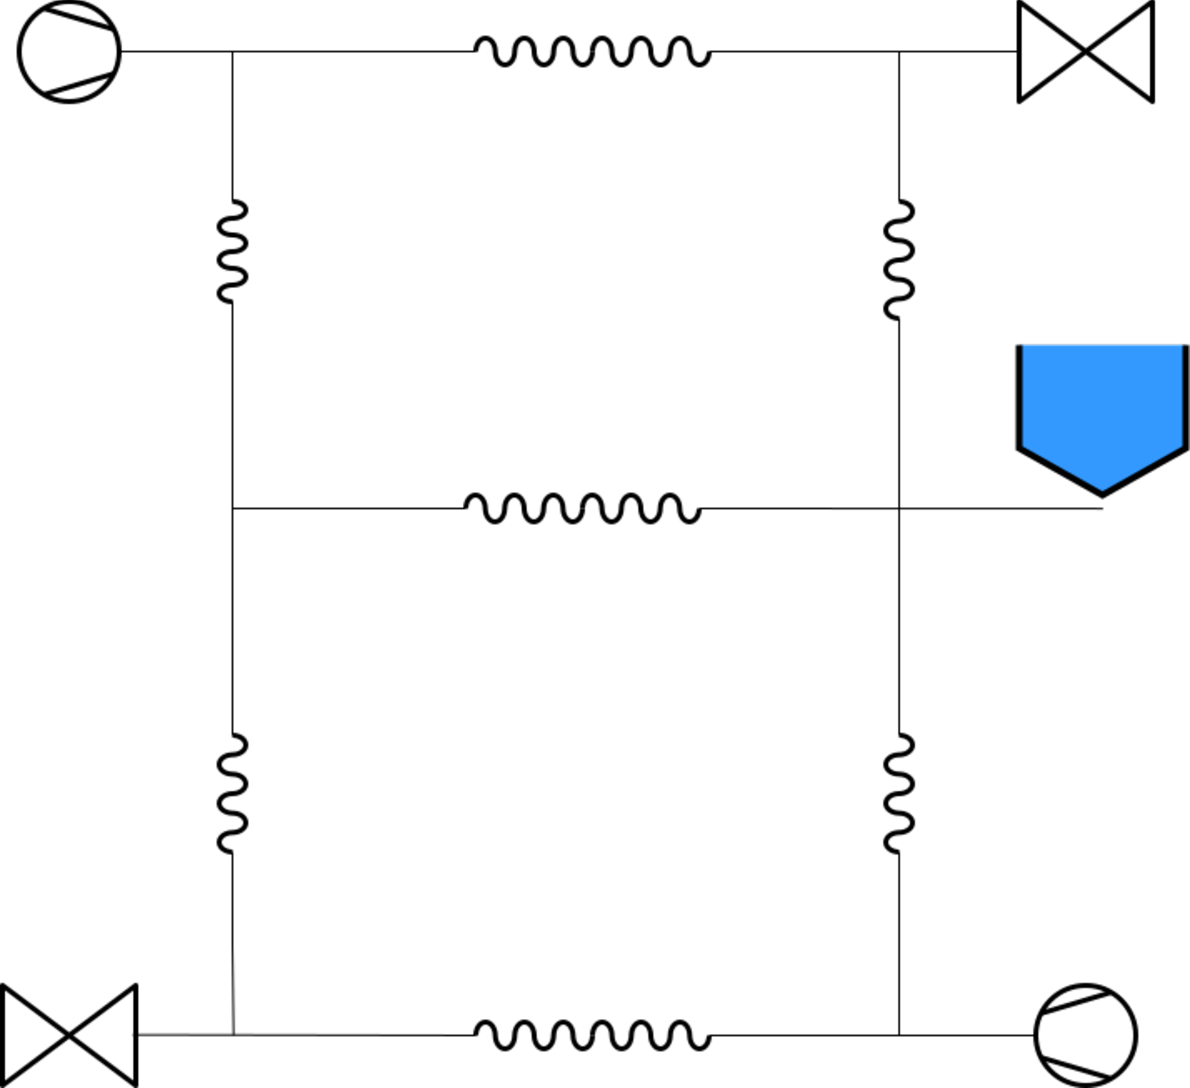
\includegraphics[width=0.5\linewidth]{Graphics/WDNModel.pdf}
	\label{fig:WDNModel}
	\begin{block}{}
		Larger WDNs are typically not amenable to first-principles modelling.
	\end{block}
\end{figure}

\end{frame}
%%%%%%%%%%%%%%%%

% ======================================================================
% Inputs for topics here!

\section{Modelling of WDN}

\begin{frame}{Modelling of WDN}
	divided in two sections..?
\end{frame}
\section{Fast Dynamics and Graph theory}

\begin{frame}{Modelling of Water Distribution Networks}
	\begin{itemize}
		\item General principles for modelling fast regime very similar to circuit analysis.
		\begin{itemize}
			\item Water flows = currents.
			\item Pressures = voltages.
			\item Network components behave similarly to circuit components, but resistors generally non-linear.
		\end{itemize}
		\item Graph theory is combined with physics-induced boundary conditions to yield model of fast regime.
	\end{itemize}
\end{frame}
% general installation instructions



\begin{frame}{Modelling of Water Distribution Networks}{Graph Theory}
	Graph theory describes a system as a directed graph.
	
	\begin{figure}[h!]
		\centering
		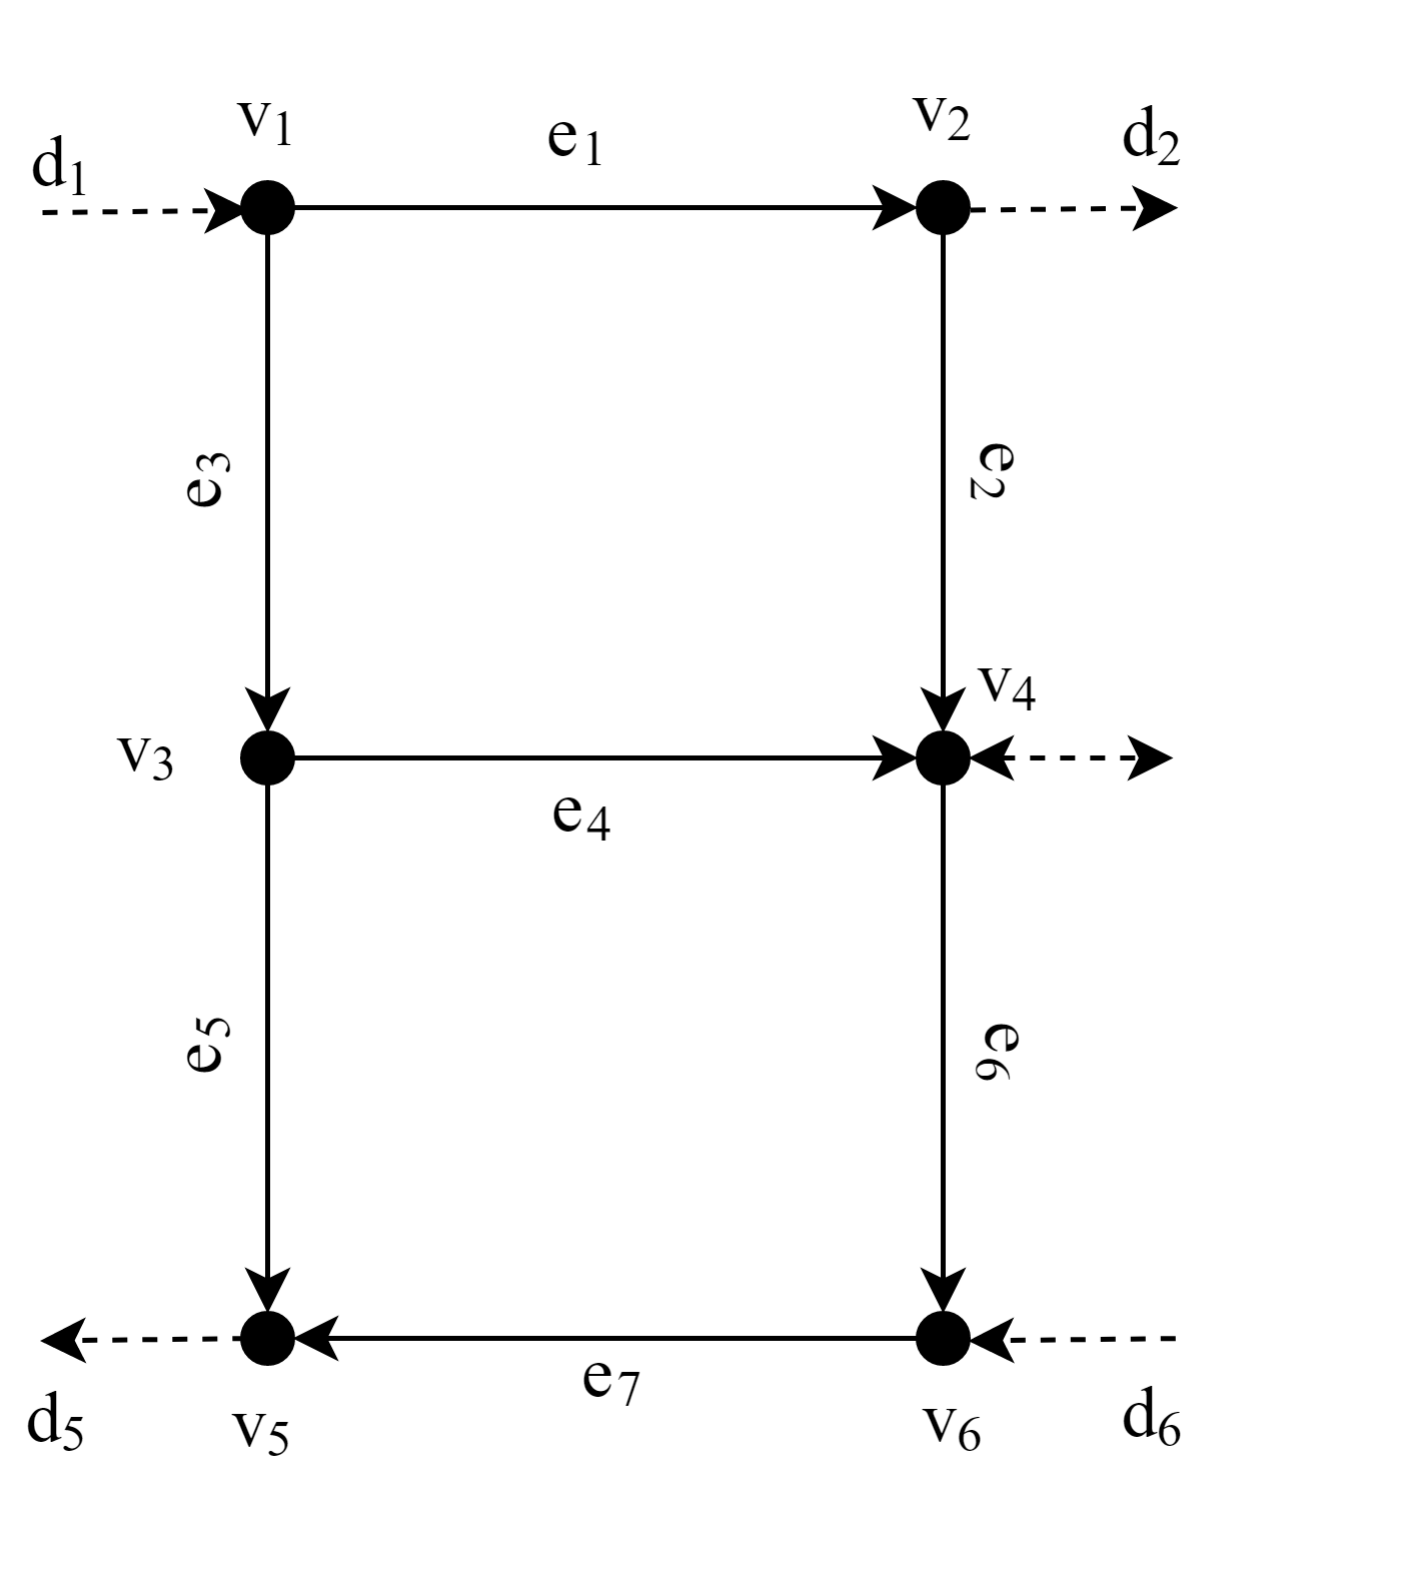
\includegraphics[width=0.4\textwidth]{Topics/SystemModel/Graphics/Graph.png}
		\caption{Graph of simplified WDN network. From \cite{Rathore930}.}
		\label{fig:graph}
	\end{figure}
	
	\begin{itemize}
		\item Spanning tree
		\item Chords
	\end{itemize}
	
\end{frame}


\begin{frame}{Modelling of Water Distribution Networks}{Incidence and Loop matrices}
Auxiliary matrices can be defined to mathematically describe the network:


\begin{equation*}
	\begin{aligned}
		&H_{i,j} = \begin{cases}
			1 & \text{If $j$th edge leaves $i$th node}\\
			-1 & \text{If $j$th edge enters $i$th node} \\
			0 & \text{If $j$th edge and $i$th node unconnected} 
		\end{cases} \\
		&B_{i,j} = \begin{cases}
			1 & \text{If direction of $ i $th loop and} \text{ $j$th edge agree}\\
			-1 & \text{If direction of $ i $th loop and} \text{ $j$th edge disagree}\\
			0 & \text{If $ i $th loop excludes $ j $th edge}\\
		\end{cases}
	\end{aligned}
\end{equation*}

\end{frame}


\begin{frame}{Modelling of Water Distribution Networks}{Incidence and Loop matrices: Example}
Example:

\begin{equation}
	H = \begin{bmatrix}
		1 & 0 & 1 & 0 & 0 & 0 & 0\\
		-1 & 1 & 0 & 0 & 0 & 0 & 0\\
		0 & 0 & -1 & 1 & 1 & 0 & 0\\
		0 & -1 & 0 & -1 & 0 & 1 & 0\\
		0 & 0 & 0 & 0 & -1 &  0  & -1\\
		0 & 0 & 0 & 0 & 0 & -1 & 1
	\end{bmatrix}
	\label{eq:H_simplified}
\end{equation} 

\begin{equation}
	\bar{H} = \begin{bmatrix}
		1 & 0 & 1 & 0 & 0 & 0 & 0\\
		-1 & 1 & 0 & 0 & 0 & 0 & 0\\
		0 & 0 & -1 & 1 & 1 & 0 & 0\\
		0 & -1 & 0 & -1 & 0 & 1 & 0\\
		0 & 0 & 0 & 0 & -1 &  0  & -1
		%0 & 0 & 0 & 0 & 0 & -1 & 1
	\end{bmatrix}
\end{equation}
\begin{equation}
	B = \begin{bmatrix}
		1 & 1 & -1 & -1 & 0 & 0 & 0\\
		0 & 0 & 0 & 1 & -1 & 1 & 1\\
	\end{bmatrix}
\end{equation}
\end{frame}


\begin{frame}{Modelling of Water Distribution Networks}{Demand Matrices}
Whether a node is open to atmosphere or not, or connected to a tank, can be described with matrices F and G respectively.
	
	
\begin{equation}
	F = \begin{bmatrix}
		1 & 0 & 0 & 0 \\
		0 & 1 & 0 & 0 \\
		0 & 0 & 0 & 0 \\
		0 & 0 & 0 & 0 \\
		0 & 0 & 1 & 0 & \\
		0 & 0 & 0 & 1 &
	\end{bmatrix}
	 , G = \begin{bmatrix}
		0  \\
		0  \\
		0  \\
		1  \\
		0 \\
		0 
\end{bmatrix}
\end{equation} 


	
\end{frame}



\begin{frame}{Modelling of Water Distribution Networks}{General Component Model}
	The edges of the WDN can be described with a pressure and flow relationship, analogous to the current and voltage of an electrical component. \\
	\medskip
	This project uses pipes, valves and pumps as edge components. \\
	\medskip
	The general relationship between pressure and flow can be defined as:
	
	\begin{equation}\label{eq:PressureFunction}
		\Delta p = \mathcal{J}\dot{q} + \lambda(q) + \mu(q, \Theta) + \alpha(q, \omega) -\Delta h
	\end{equation}
	
	
\end{frame}




\begin{frame}{Modelling of Water Distribution Networks}{Pipe Model}
The pressure drop across a pipe is defined as:

	\begin{equation}
		\Delta{p_{k}} = \mathcal{J}\dot{q} + \lambda(q) + \Delta z
	\end{equation}

where:

	\begin{equation}
		\lambda_{k}(q_{k})  =	\Big(f \cdot \frac{8\cdot L\cdot q^{2}}{\pi^{2}\cdot g \cdot D^{5}} + k_{f}\cdot \frac{8\cdot q^{2}}{\pi^{2}\cdot g \cdot D^{4}}\Big)\cdot g \cdot \rho
	\end{equation}
	
	
	\begin{equation}
		\mathcal{J} = \frac{L\cdot \rho}{A}
	\end{equation}
	
	\begin{equation}
		\Delta{z_{k}} = \rho \cdot g \cdot \Delta{h_{k}}
	\end{equation}
\end{frame}



\begin{frame}{Modelling of Water Distribution Networks}{Valve Model}
	The pressure drop across a valve is defined as:
	\begin{equation}\label{eq:ValvePressure}
		\Delta p_{k} = \mu(q,\Theta) = \frac{1}{K_{valve}(\Theta)^2} \cdot |q|\cdot q 
	\end{equation}
	
	where $\Theta$ is the opening degree of the valve.\\
	
	Derivation:
	
	\begin{equation}\label{eq:HydrodynamicRatio}
		\frac{\Delta p_1}{q_1^2} = \frac{\Delta p_2}{q_2^2} 	\Leftrightarrow
		q_1 = q_2\cdot\sqrt{\frac{\Delta p_1}{\Delta p_2}}
	\end{equation}
\begin{equation}\label{eq:Kvalve}
	q = q_n(\Theta)\cdot\sqrt{\frac{\Delta p_1}{1}} = K_{valve}(\Theta)\cdot\sqrt{\Delta p_1}
\end{equation}
\end{frame}


\begin{frame}{Modelling of Water Distribution Networks}{Pump Model}
	The pressure drop across a pump is defined as:
	\begin{equation}\label{eq:PumpPressure}
		\Delta p_{k} =   a_0\cdot \omega^2 +  a_1\cdot \omega \cdot q -a_2\cdot |q|\cdot q
	\end{equation}
	
	where $[a_0,a_1,a_2]$ is a tuple of coefficients that describe the pump's characteristic curve, $q$ is the flow rate through the pump, and $\omega$ is the rotational velocity of the pump.
	
\end{frame}




\begin{frame}{Modelling of Water Distribution Networks}{Assumptions}
	Kirchhoff's node and mesh law:
	
	\begin{equation}
		Hq = d  
	\end{equation} 
	\begin{equation}
		B\Delta p = B H^T p = 0 \wedge B\Delta h = B H^T h = 0 
	\end{equation} 

	Mass conservation:
	\begin{equation}\label{eq:MassConservation}
		d_n = -\sum_{i=1}^{n-1}d_i
	\end{equation}
\end{frame}


\begin{frame}{Modelling of Water Distribution Networks}{Lemmas}
	Lemma 4.1:
	\begin{equation}\label{eq:TreePartitionLemma}
		H_T\bar{H}_T^{-1} = \begin{bmatrix} I_{n-1} \\ -\mathbf{1}^T	\end{bmatrix}
	\end{equation}
	where $\mathbf{1}$ is a vector of ones and $I_{n-1} \in \mathbb{R}^{n-1 \times n-1}$ is an identity matrix.


	Lemma 4.2:
	\begin{equation}\label{eq:EdgeFlowDecomposition}
		q = B^T q_C +
		\begin{bmatrix}
			0_{C \times n-1} \\ \bar{H}_T^{-1} 
		\end{bmatrix}
		\bar{d}
	\end{equation}

\end{frame}


\begin{frame}{Modelling of Water Distribution Networks}{System Model}
	Non linear differential equation:
	\begin{equation}
		\Phi\mathcal{J}\Phi^T \dot{q} = -\Phi\Big(\lambda(q_n)+\mu(q_n)+\alpha(q_n)\Big) + \Psi(\bar{h}-\mathbf{1}h_0) + \mathcal{I}(p_{\tau}-\mathbf{1}p_0)
	\end{equation}

	Where the matrices $\Phi, \Psi, \mathcal{I}$ are defined as:
	
	\begin{equation}
		\Phi \triangleq 
		\begin{bmatrix} 
			I & -\bar{H}_C^T\bar{H}_T^{-T} \\ 0 & \bar{F}^T\bar{H}_T^{-T} \\ 0  & \bar{G}^T\bar{H}_T^{-T} \\ 
		\end{bmatrix}
		, \qquad
		\Psi \triangleq
		\begin{bmatrix}
			0 \\ \bar{F}^T \\ \bar{G}^T
		\end{bmatrix}
		, \qquad
		\mathcal{I} \triangleq
		\begin{bmatrix}
			0 \\ 0 \\ I
		\end{bmatrix}
	\end{equation}

	\begin{equation}
		\mathcal{P}: (\Phi \mathcal{J} \Phi^T)^{-1}
	\end{equation}
	
	
	
	\begin{equation}\label{eq:NonLinearModelSimplified}
		\begin{split}
			\dot{q}_n &=  -\mathcal{P}\Phi\Big(\lambda(q_n)+\mu(q_n)+\alpha(q_n)\Big) + \mathcal{P}\Big(\Psi(\bar{h}-\mathbf{1}h_0) + \mathcal{I}(p_{\tau}-\mathbf{1}p_0)\Big) 
		\end{split}	
	\end{equation}

\end{frame}

\begin{frame}{Modelling of Water Distribution Networks}{System Model Simulation}
	
	\movie[externalviewer]{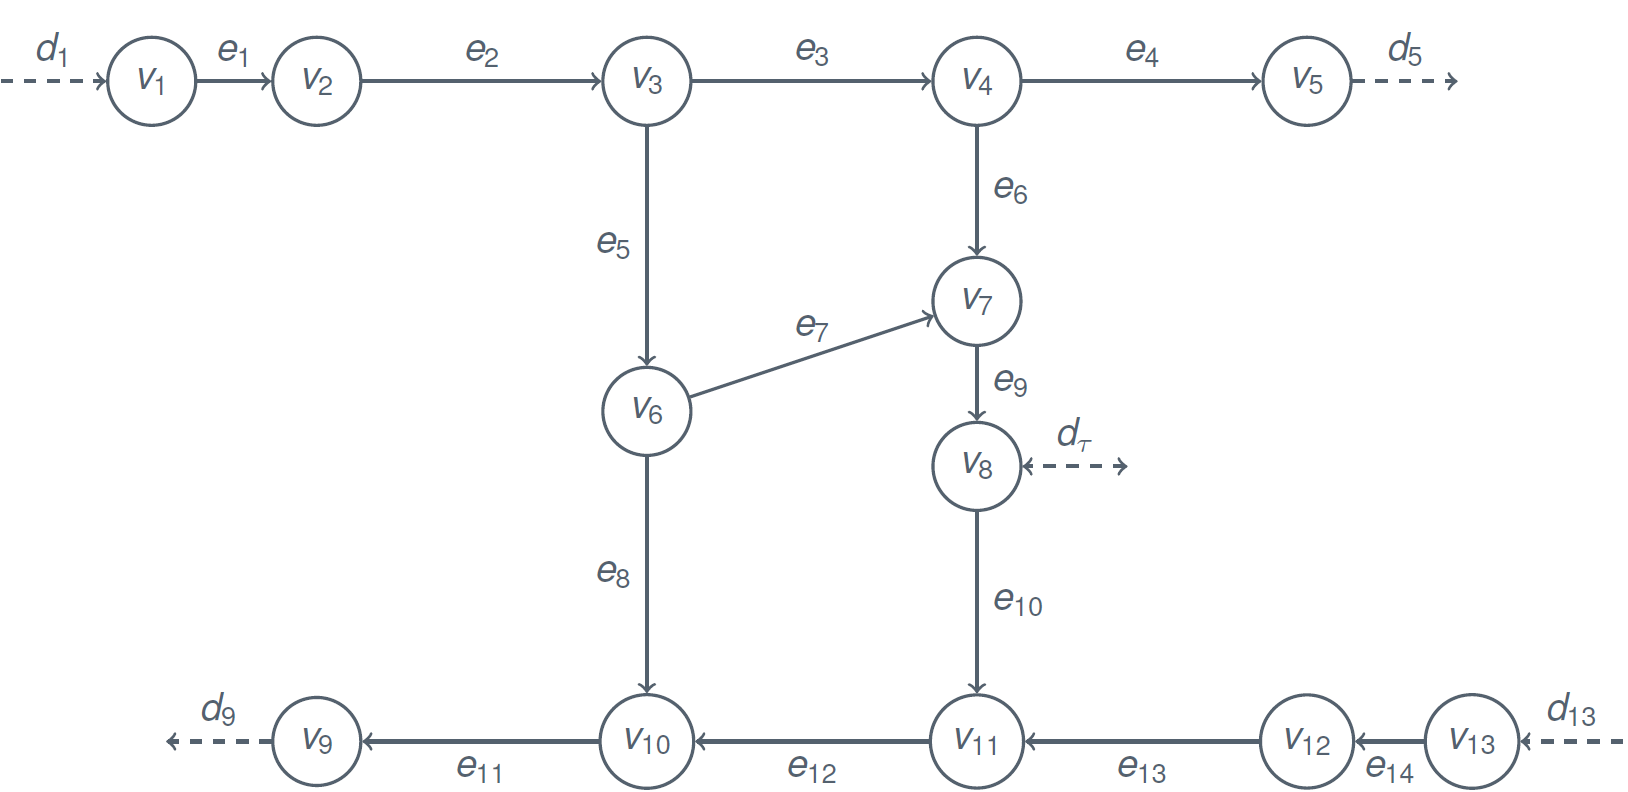
\includegraphics[width=\textheight,keepaspectratio]{Topics/SystemModel/Graphics/Graph_sim.png}}{Topics/SystemModel/Graphics/Simulering.mp4}
	
\end{frame}

%
\section{Slow Dynamics and Linearisation}
\subsubsection{Slow Dynamics}

\begin{frame}{Modelling of Water Distribution Networks}{Slow Dynamics}
	\begin{columns}
		\begin{column}{.5\textwidth}
			\begin{itemize}
				\item Fundamentals
				\begin{equation*}
					p \propto h 
				\end{equation*}
				\begin{equation*}
					\dot{V} = q
				\end{equation*}
				\item Assume constant cross sectional area A
				\begin{equation*}
					V \propto h \implies V \propto p 
				\end{equation*}
				\begin{equation*}
					\dot{p} \propto \dot{V} \wedge \dot{V} = q \implies \dot{p} \propto q
				\end{equation*}
				\item We arrive at
				\begin{equation*}
					\dot{p} = -\tau q \text{,  where}
				\end{equation*}	
				\begin{equation*}
					\tau = \rho g \frac{1}{A}
				\end{equation*}	
			\end{itemize}
		\end{column}
		\begin{column}{.5\textwidth}\raggedleft
			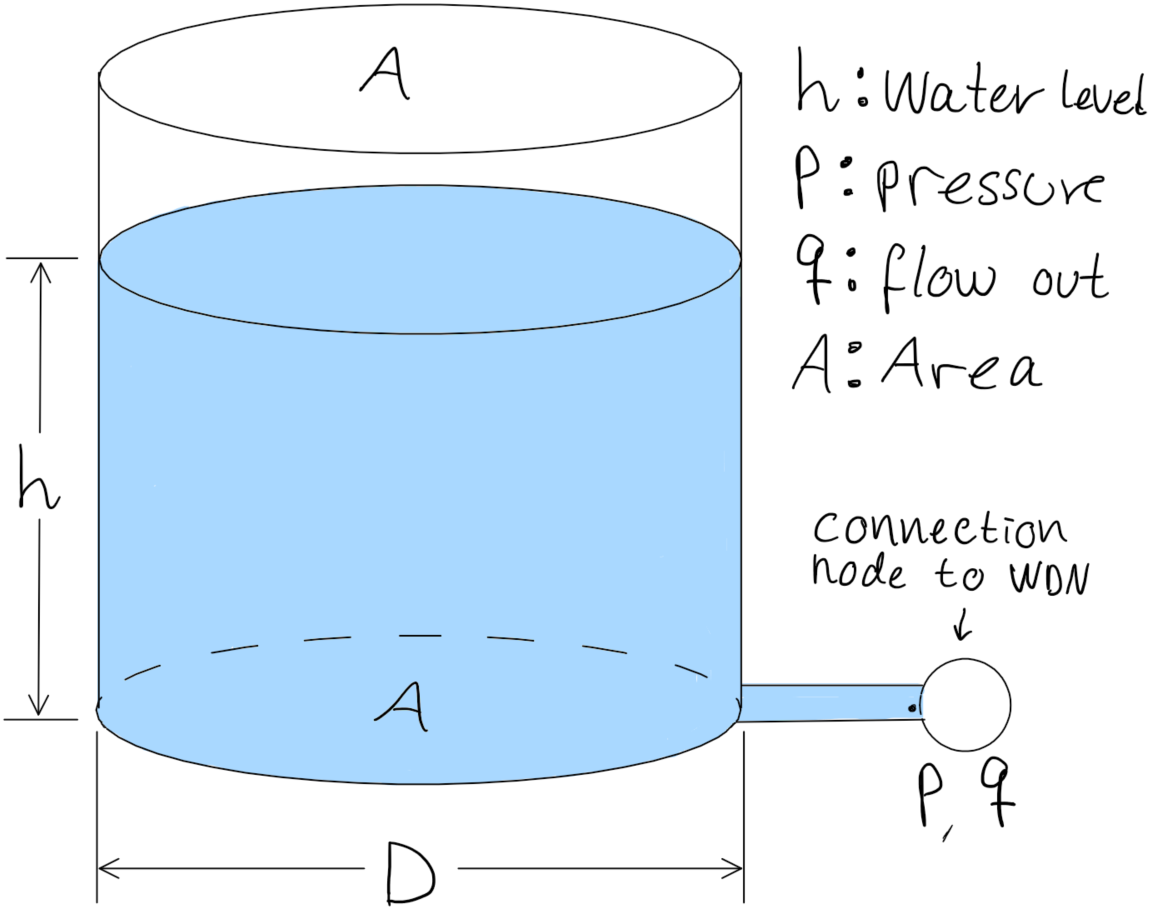
\includegraphics[width=1\linewidth]{Topics/SlowDynamicsLinearisation/Graphics/Tank_sketch.png}
		\end{column}
	\end{columns}
\end{frame}

\begin{frame}{Modelling of Water Distribution Network}{State-space Formulation of Slow Dynamics}
	\begin{figure}[h!]
		\centering
		\resizebox{\columnwidth}{!}{
				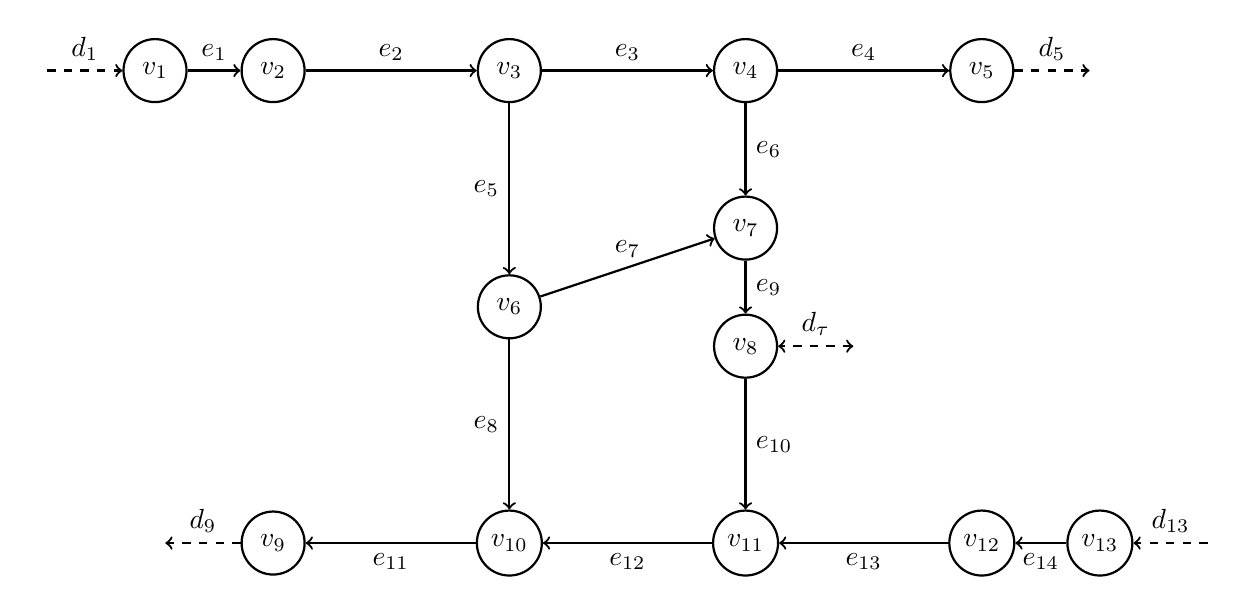
\begin{tikzpicture}[node distance=30mm, thick, main/.style = {draw,circle,minimum size=0.8cm}] 
		\node (1)  {};
		\node[main] (2) [node distance={15mm},right of=1] {$v_1$}; 
		\node[main] (3) [node distance={1.5cm},right of=2] {$v_2$};
		\node[main] (4) [right of=3] {$v_3$};
		\node[main] (5) [right of=4] {$v_4$};
		\node[main] (6) [right of=5] {$v_5$};
		\node (7) [node distance={15mm},right of=6] {};
		%Create 3 (4) nodes in middle part of graph
		\node[main] (8) [below of=4] {$ v_6 $};
		\node[main] (9) [node distance={20mm},below of=5] {$ v_7 $};
		\node[main] (11) [node distance={15mm},below of=9] {$ v_8 $};
		\node (10) [node distance={15mm},right of=11] {};
		%First 5 (7) nodes in bottom part of graph
		\node[main] (12) [below of=8] {$ v_{10} $};
		\node[main] (13) [left of=12] {$ v_9 $};
		\node(14) [node distance={15mm},left of=13] {};
		\node[main] (15) [right of=12] {$ v_{11} $};
		\node[main] (16) [right of=15] {$ v_{12} $};
		\node[main] (17) [node distance={1.5cm},right of=16] {$ v_{13} $};
		\node(18) [node distance={15mm},right of=17] {};
		
		%Edges with direction
		\path [->] (2) edge node[above] {$e_{1}$} (3); 	%Edge v1 -> v2
		\path [->] (3) edge node[above] {$e_{2}$} (4); 	%Edge v2 -> v3
		\path [->] (4) edge node[above] {$e_{3}$} (5); 	%Edge v3 -> v4
		\path [->] (5) edge node[above] {$e_{4}$} (6); 	%Edge v4 -> v5
		
		\path [->] (4) edge node[left] {$e_{5}$} (8); 	%Edge v3 -> v6
		\path [->] (5) edge node[right] {$e_{6}$} (9); 	%Edge v4 -> v7
		\path [->] (8) edge node[above] {$e_{7}$} (9); 	%Edge v6 -> v7
		\path [->] (8) edge node[left] {$e_{8}$} (12); 	%Edge v6 -> v10
		\path [->] (9) edge node[right] {$e_{9}$} (11); 	%Edge v7 -> v8
		\path [->] (11) edge node[right] {$e_{10}$} (15);	 %Edge v8 -> v11
		
		
		\path [->] (12) edge node[below] {$e_{11}$} (13); %Edge v10 -> v9
		\path [->] (15) edge node[below] {$e_{12}$} (12); %Edge v11 -> v10
		\path [->] (16) edge node[below] {$e_{13}$} (15); %Edge v12 -> v11
		\path [->] (17) edge node[below] {$e_{14}$} (16); %Edge v13 -> v12
		
		%External flows
		\draw[->,dashed,] (1) -- node[above] {$d_1$} (2); %Create d1
		\draw[->,dashed,] (6) -- node[above] {$d_5$} (7); %Create d5
		\draw[->,dashed,] (13) -- node[above] {$d_9$} (14); %Create d13
		\draw[->,dashed,] (18) -- node[above] {$d_{13}$} (17); %Create d13
		\draw[<->,dashed,] (10) -- node[above] {$d_\tau$} (11); %Create d_tau
	\end{tikzpicture} }
		\label{fig:tikzWDNGraph}
	\end{figure}  
	In context of WDN we now consider flows to and from network as external demands $ d_i $
\end{frame}

\begin{frame}{Modelling of Water Distribution Networks}{State-space Formulation of Slow Dynamics}
	Mass conservation holds, and such
	\begin{equation*}
		d_n = -\sum_{i=1}^{n-1}d_i \implies d_\tau = - (d_p + d_c)
	\end{equation*}
	\begin{equation*}
		\dot{p} = -\tau d_\tau = \tau (d_p + d_c)
	\end{equation*}	
	When discretised by forward Euler:
	\begin{equation*}
		p_\tau(k+1) = p_\tau(k) - \tau d_\tau(k) t_s = p_\tau(k) + \tau(d_p(k) + d_c(k)) t_s
	\end{equation*}
	Which corresponds to a discrete, linear state-space model:
	\begin{equation}
		p_\tau(k+1) = Ap_\tau(k) + B_pd_p(k) + B_cd_c(k)
	\end{equation}
	\begin{equation*}
		d_p = \begin{bmatrix}
			d_1 \\ d_{13}
		\end{bmatrix},
		d_c = \begin{bmatrix}
			d_5 \\ d_9
		\end{bmatrix},
		B_p = B_c = t_s  \begin{bmatrix}
			\tau & \tau
		\end{bmatrix},
		A = 1
	\end{equation*}
\end{frame}


\subsubsection{Linearisation}
\begin{frame}{Modelling of Water Distribution Networks}{Linearisation}
	\begin{columns}
		\begin{column}{.4\textwidth}
			\begin{itemize}
				\item Fast dynamics are non-linear
				\item Linearisation required
			\end{itemize}
			In near vicinity of linearisation point $ x_0 $,
			\begin{equation*}
				\dot{x} \approx f(x_0) + \nabla f\bigg\rvert_{x_0} (x-x_0)
			\end{equation*}
			Linearising around equilibrium point preferred
		\end{column}
		\begin{column}{.6\textwidth}\raggedleft
			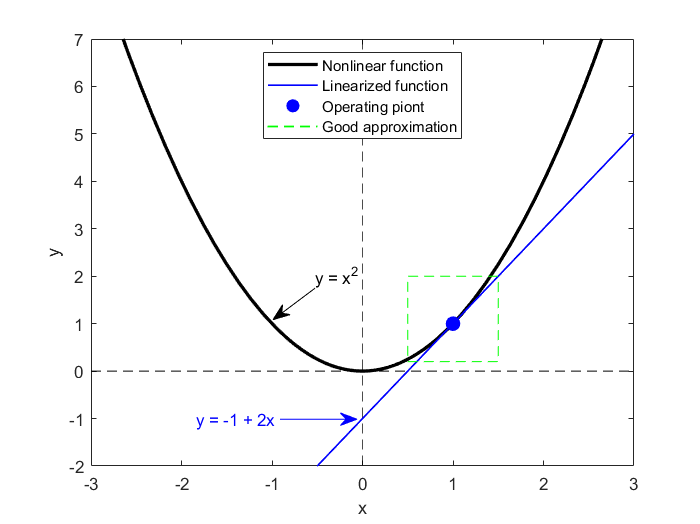
\includegraphics[width=1\linewidth]{Topics/SlowDynamicsLinearisation/Graphics/Linearisation_pic.png}
		\end{column}
	\end{columns}
\end{frame}

\begin{frame}{Modelling of Water Distribution Networks}{Linearisation}
%	Fast dynamics are non linear - linearisation is needed.\\
%	In near vicinity of linearisation point $ x_0 $,
%	\begin{equation*}
%		\dot{x} \approx f(x_0) + \nabla f\bigg\rvert_{x_0} (x-x_0)
%	\end{equation*}
	Recalling the fast dynamics differential equation is given as
	\begin{equation}\label{eq:NonLinearModelSimplified}
		\begin{split}
			\dot{q}_n &=  -\mathcal{P}\Phi\Big(\lambda(q_n)+\mu(q_n,\Theta)+\alpha(q_n,\omega)\Big) +\\ &\mathcal{P}\Big(\Psi(\bar{h}-\mathbf{1}h_0) + \mathcal{I}(p_{\tau}-\mathbf{1}p_0)\Big) \\
		\end{split}	
	\end{equation}
	The linear model such becomes
	\begin{equation}\label{eq:SymbolicLinearisation}
		\begin{split}
			\dot{q}_n &\approx f(x_0) + \frac{\partial f}{\partial q_n}\bigg\rvert_{x_0} \tilde{q}_n + \frac{\partial f}{\partial \Theta}\bigg\rvert_{x_0} \tilde{\Theta} + \frac{\partial f}{\partial \omega}\bigg\rvert_{x_0} \tilde{\omega} +  \frac{\partial f}{\partial p_\tau}\bigg\rvert_{x_0} \tilde{p}_\tau
			\\
		\end{split}
	\end{equation}
	where $x_0 = \{q_0,\Theta_0,\omega_0, p_{\tau_0} \}$, $ \tilde{q} =q-q_0$, likewise for $ \tilde{\Theta} $, $ \tilde{\omega}$, $\tilde{p_{\tau}}  $
\end{frame}

\begin{frame}{Modelling of Water Distribution Networks}{Linearisation}
	The full linearised model is then obtained as
	\begin{equation}\label{eq:SymbolicLinearisationExpanded}
		\begin{split}
			\dot{q}_n \approx f(x_0) -\mathcal{P}\Phi & \Bigg(a_1\omega_0 + \Big(|q_0|+\text{sign}(q_0)q_0\Big)\\
			& \Bigg(K_\lambda + a_2 + \frac{1}{(K_v \Theta_0)^2}\Bigg) \tilde{q}_n \Bigg)  \\
			- \mathcal{P}\Phi&\Bigg(\Big(-|q_0|q_0 \frac{2}{K_v^2 \Theta_0^3}\Big) \tilde{\Theta}\Bigg) \\
			- \mathcal{P}\Phi&\Bigg(\Big(a_1 q_0 + 2a_0\omega_0\Big) \tilde{\omega}\Bigg) \\
			+ \mathcal{P} \mathcal{I}& \tilde{p}_\tau
		\end{split}
	\end{equation}
The equation can be simplified further making some assumptions
\end{frame}

\begin{frame}{Modelling of Water Distribution Networks}{Linearisation}
	Equilibrium disappears, valve and tank dynamics assumed to be constant disturbances 
	\begin{equation}\label{eq:SymbolicLinearisationSimplified}
		\begin{split}
			\dot{q}_n \approx -\mathcal{P}\Phi &\Bigg(a_1\omega_0 + \Big(|q_0|+\text{sign}(q_0)q_0\Big) \\
			&\Bigg(K_\lambda + a_2 + \frac{1}{(K_v \Theta_0)^2}\Bigg) \tilde{q}_n \Bigg) \\
			- \mathcal{P}\Phi&\Bigg(\Big(a_1 q_0 + 2a_0\omega_0\Big) \tilde{\omega}\Bigg)
		\end{split}
	\end{equation}
	
\end{frame}

%
\section{Control structure and root locus}

\begin{frame}{Control Structure}
	We elect for a cascaded control structure with optimal central control and local PI control.
	\begin{figure}[h!]
		\centering
		\resizebox{\columnwidth}{!}{
				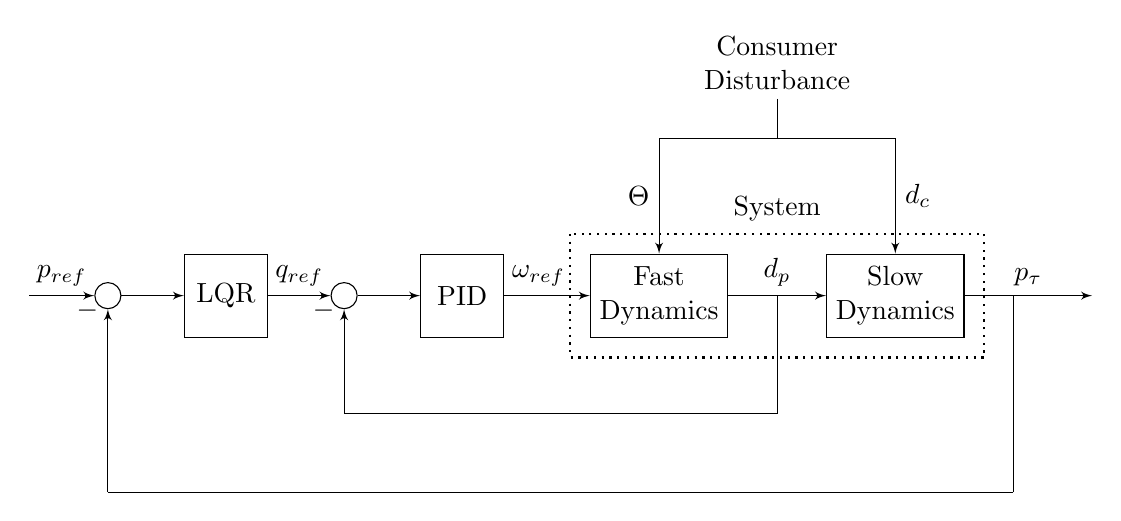
\begin{tikzpicture}[auto, node distance=2.5cm,>=latex']
	% ========================== Nodes ============================
	% Nodes in upper vertical line
	\node [input, name=rinput] (rinput) {};
	\node [sum, right of=rinput] (sum1) {};
	\node [block, right of=sum1, node distance = 1.5cm] (LQR) {LQR};
	\node [sum, right of=LQR, node distance =
	1.5cm] (sum2) {};
	\node [block, right of=sum2, node distance = 1.5cm] (PID){PID};
	\node [block, right of=PID, align=center] (Fast){Fast\\Dynamics};
	\node [block, right of=Fast, node distance = 3cm, align=center] (Slow){Slow\\Dynamics};
	\node [output, right of=Slow] (output) {};
	
	% Nodes for inner feedback
	\node [tmp, right of=Fast, node distance = 1.5cm] (tmp0){};
	\node [tmp, below of=tmp0, node distance = 1.5cm] (tmp1){};
	\node [tmp, below of=sum2, node distance = 1.5cm] (tmp2){};
	
	% Nodes for outer feedback
	\node [tmp, right of=Slow, node distance = 1.5cm] (tmp10){};
	\node [tmp, below of=tmp10,node distance = 2.5cm] (tmp11){};
	\node [tmp, below of=sum1, node distance = 2.5cm] (tmp12){};
	
	% Nodes for Disturbance
	\node [tmp, above of=tmp0, node distance = 2.5cm] (tmp20){};
	\node [tmp, above of=tmp0, node distance = 2cm] (tmp21){};
	\node [tmp, above of=Fast, node distance = 2cm] (tmp22){};
	\node [tmp, above of=Slow, node distance = 2cm] (tmp23){};
	
	\draw[thick, dotted] ($(Fast.north west)+(-0.25, 0.25)$) rectangle  ($(Slow.south east)+(0.25, -0.25)$);
	\node[above of =tmp0, node distance =1.1cm](sys_txt) {System};
	
	% ========================== Lines ============================
	
	% Lines in upper vertical part of block diagram
	\draw [->] (rinput) -- node{$p_{ref}$} (sum1);
	\draw [->] (sum1) --node[name=z,anchor=north]{} (LQR);
	\draw [->] (LQR) -- node{$ q_{ref} $}(sum2);
	\draw [->] (sum2) -- (PID);
	\draw [->] (PID) -- node[pos=0.4]{$ \omega_{ref} $}(Fast);
	\draw [->] (Fast) -- node{$d_p$}(Slow);
	\draw [->] (Slow) -- node{$p_{\tau}$}(output);	
	
	% Lines for inner feedback
	\draw [-] (tmp0) -- (tmp1);
	\draw [-] (tmp1) -- (tmp2);
	\draw [->] (tmp2) -- node[pos=0.99]{$ - $}(sum2);
	
	
	% Lines for outer feedback
	\draw [-] (tmp10) -- (tmp11);
	\draw [-] (tmp11) -- (tmp12);
	\draw [->] (tmp12) -- node[pos=0.99]{$ - $}(sum1);
	
	
	% Lines for disturbance
	\draw [-] (tmp20)node[above, align=center]{Consumer \\ Disturbance} -- (tmp21);
	\draw [-] (tmp21) -- (tmp22);
	\draw [-] (tmp21) -- (tmp23);
	\draw [->] (tmp22) -- node[left, pos = 0.5]{$\Theta$}(Fast);
	\draw [->] (tmp23) -- node[pos = 0.5]{$ d_c $}(Slow);
	
	
\end{tikzpicture}
}
		\label{fig:tikzControlStrat}
	\end{figure}
\end{frame}

\begin{frame}{Control Structure}{The Root Locus Method}
	\begin{figure}[h]
		\centering
		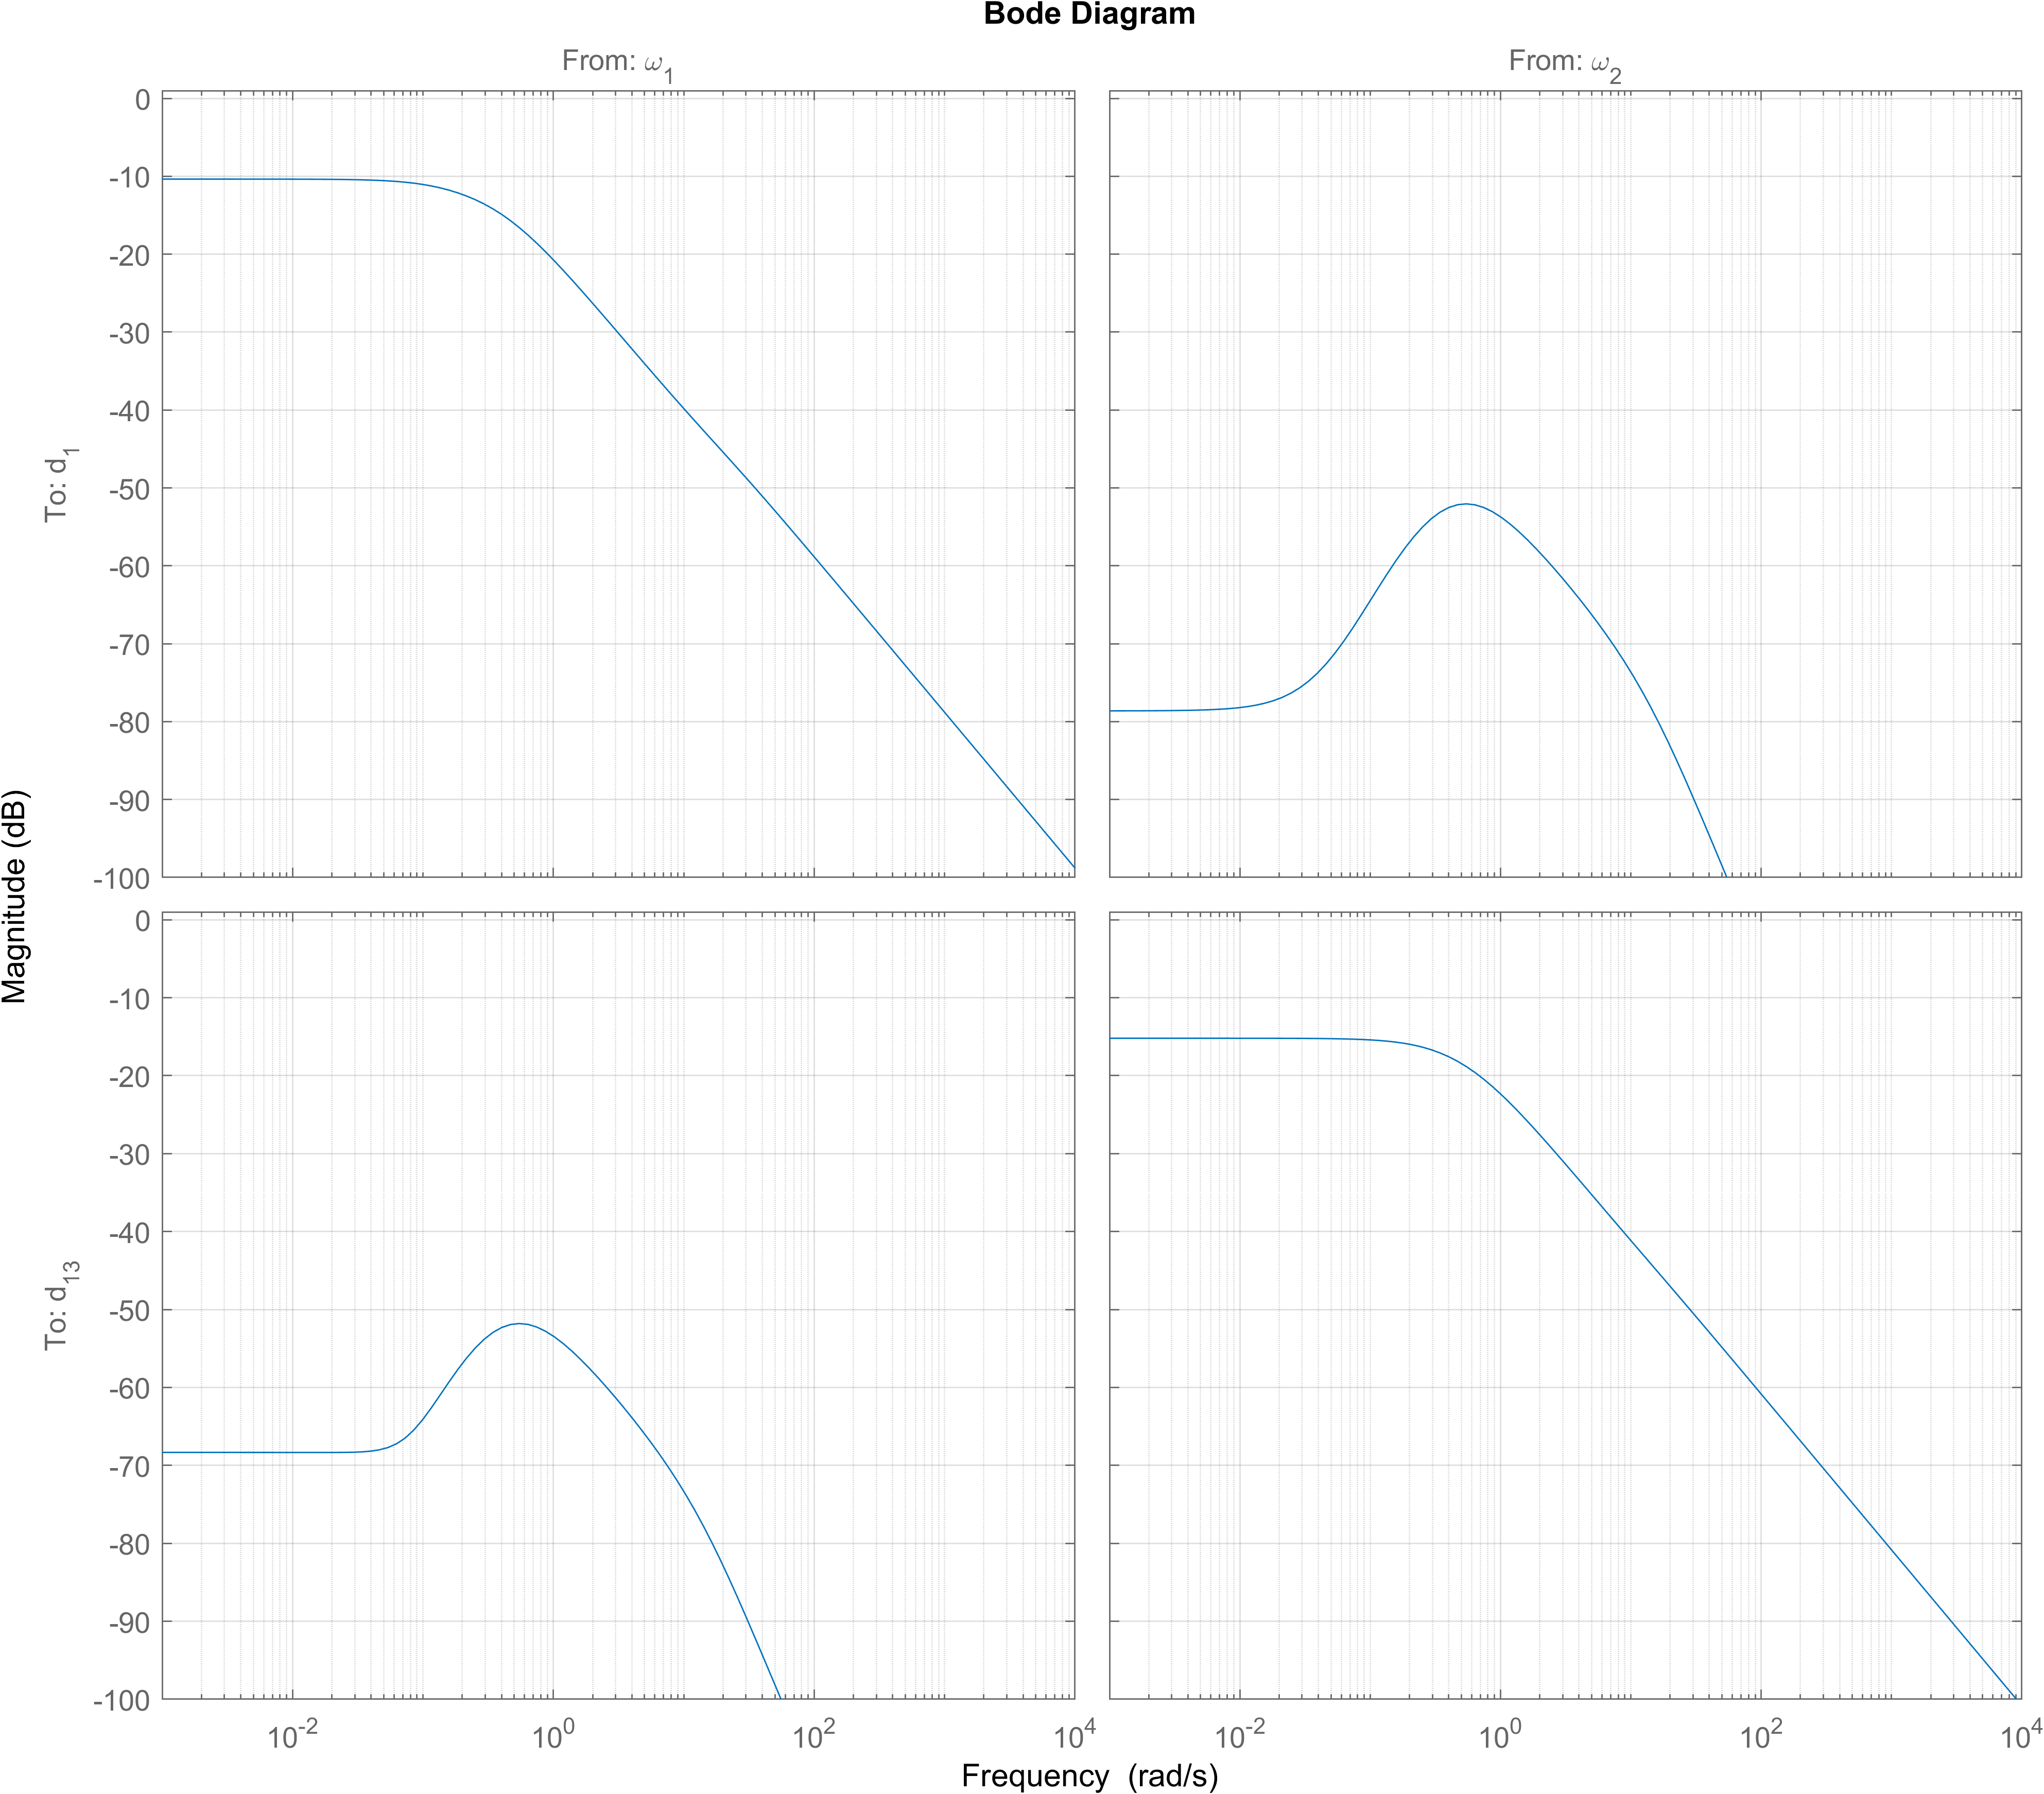
\includegraphics[width=0.75\linewidth]{Topics/ControlStructure/Graphics/PumpMagPlot.png}
		\label{fig:PumpMagPlot}
	\end{figure}
\end{frame}

\begin{frame}{Control Structure}{The Root Locus Method}

	\begin{figure}[h]
		\centering
		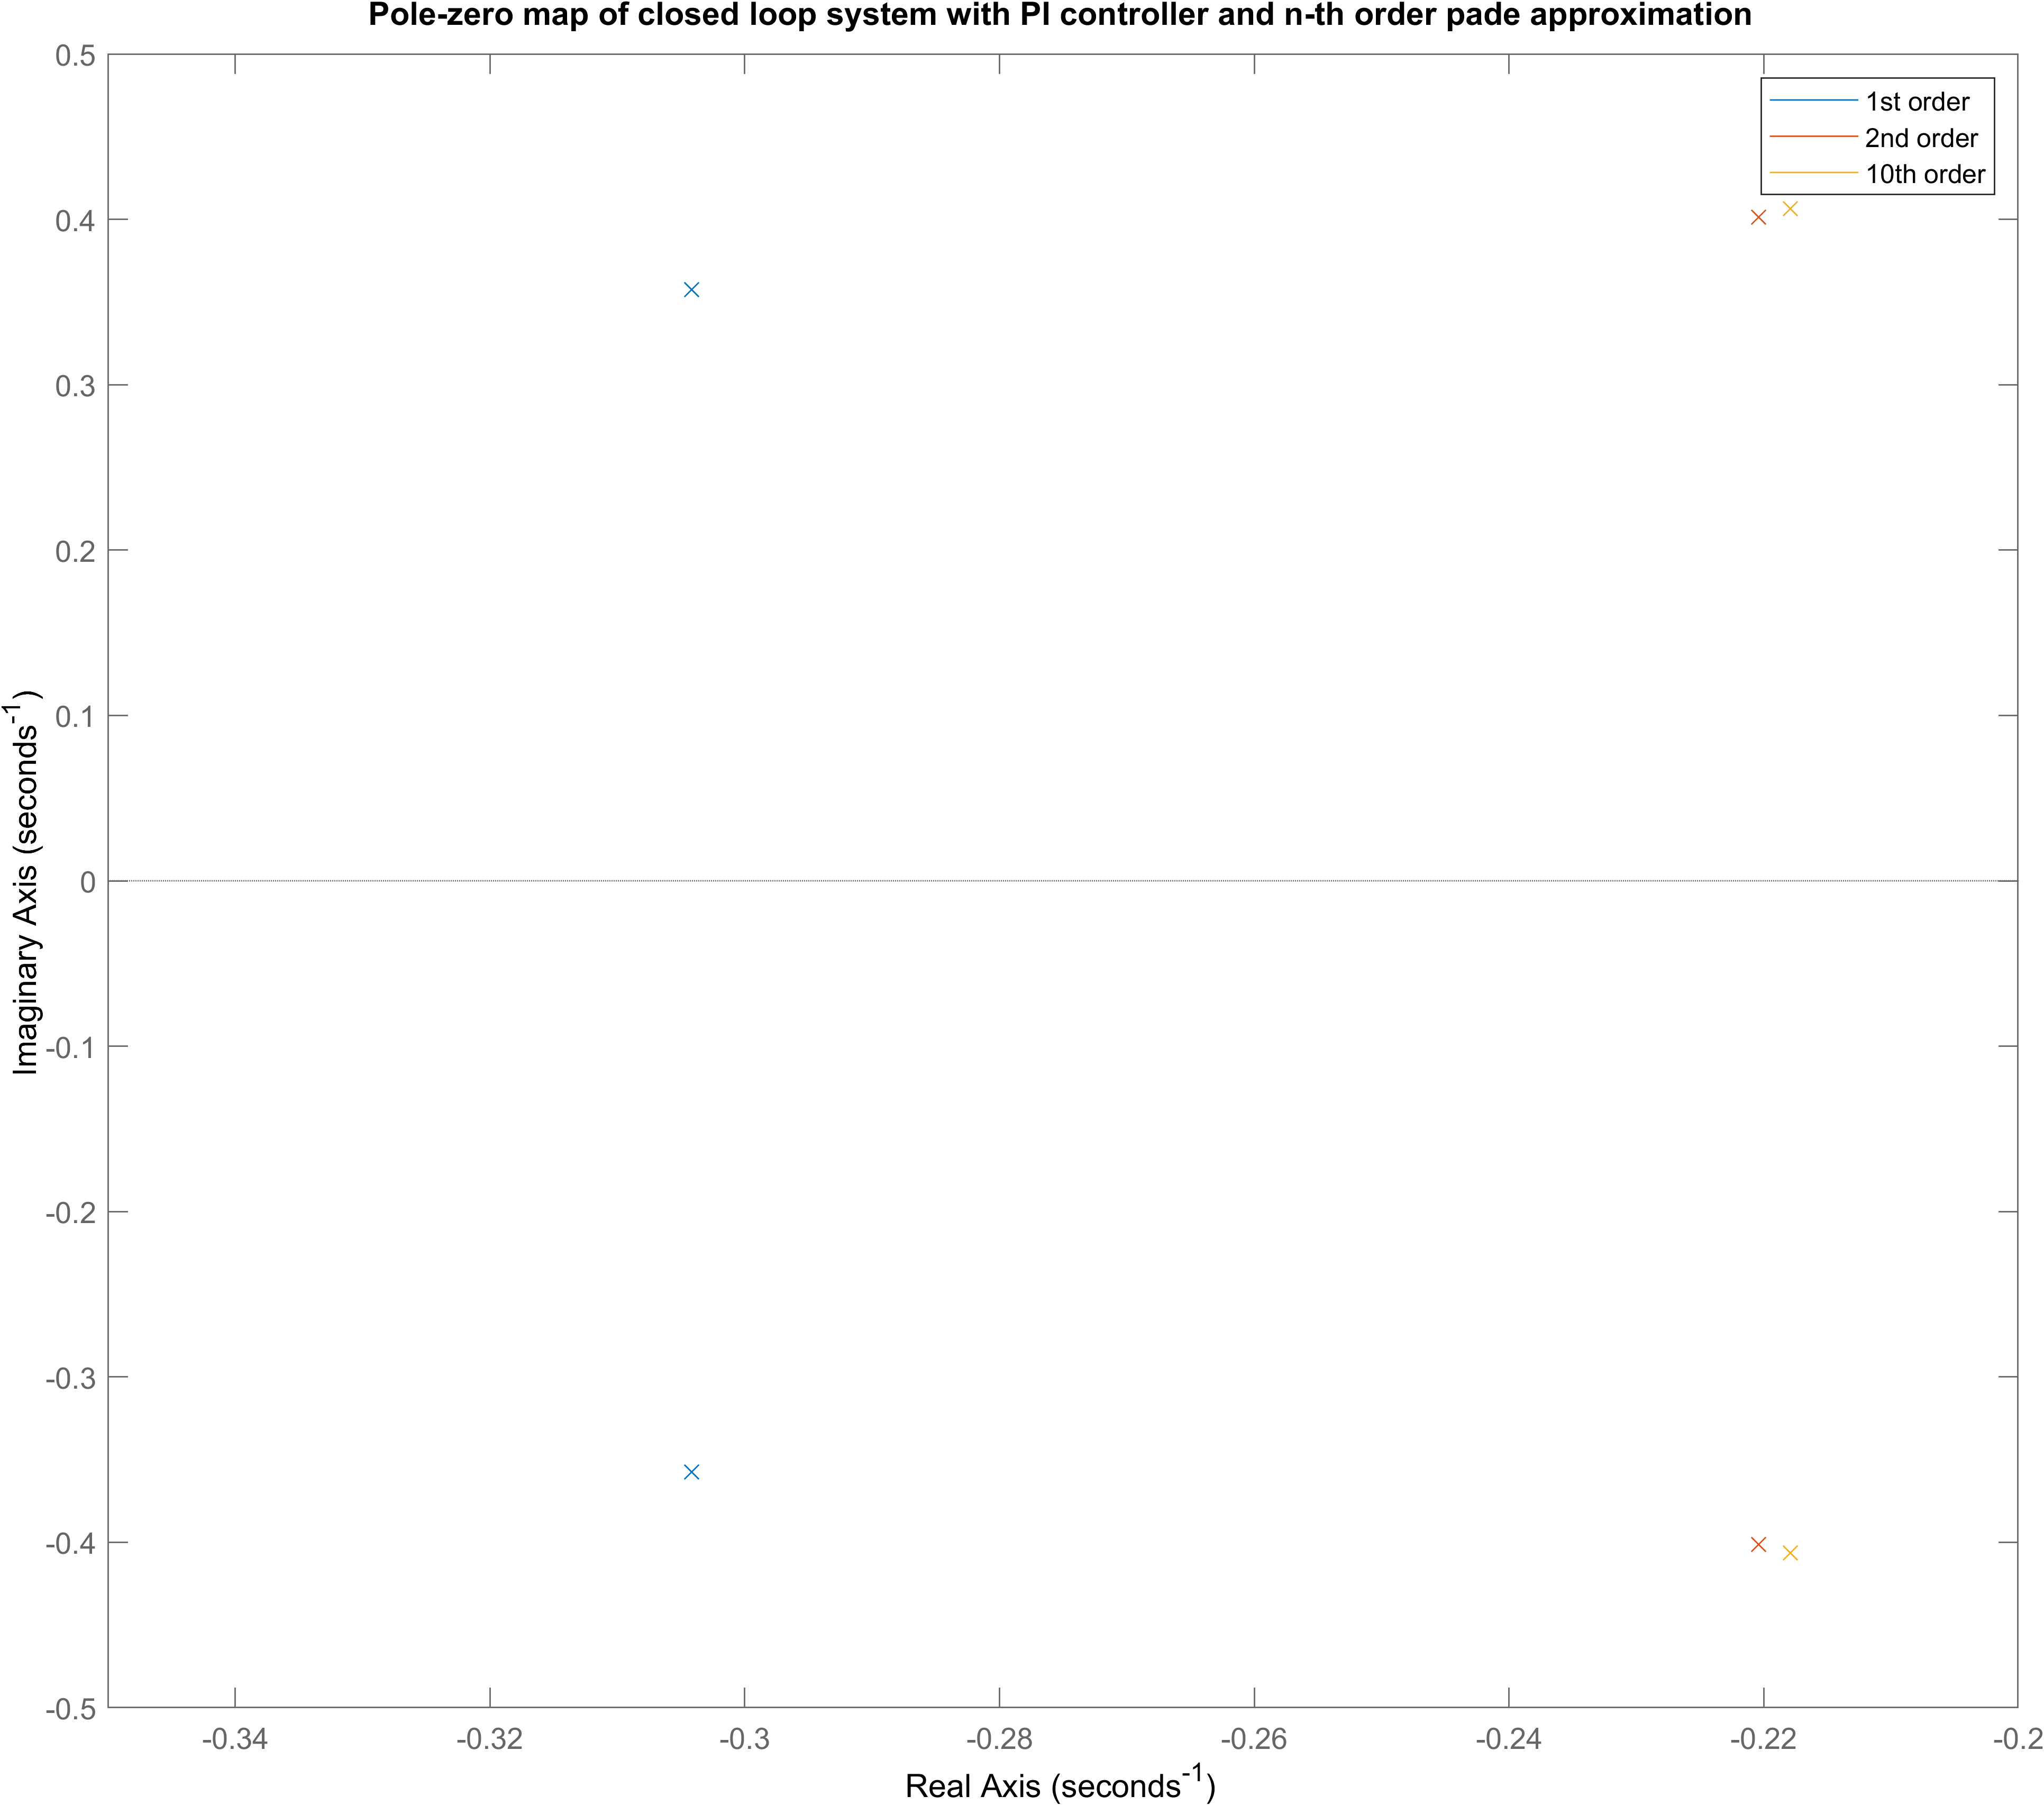
\includegraphics[width=0.75\linewidth]{Topics/ControlStructure/Graphics/PZmap_CL_zoom.png}
		\label{fig:PZmap_CL_zoom}
	\end{figure}
\end{frame}


\begin{frame}{Control Structure}{Root Locus and Resulting Controller}
\begin{columns}
	\begin{column}{.4\textwidth}
			\begin{itemize}
			\item Faster than outer loop.\\
			\item No steady state error.\\
			\item No overshoot, and low amount of oscillation.\\
			\item Stability.
		\end{itemize}
	\end{column}
	\begin{column}{.6\textwidth}\raggedleft
		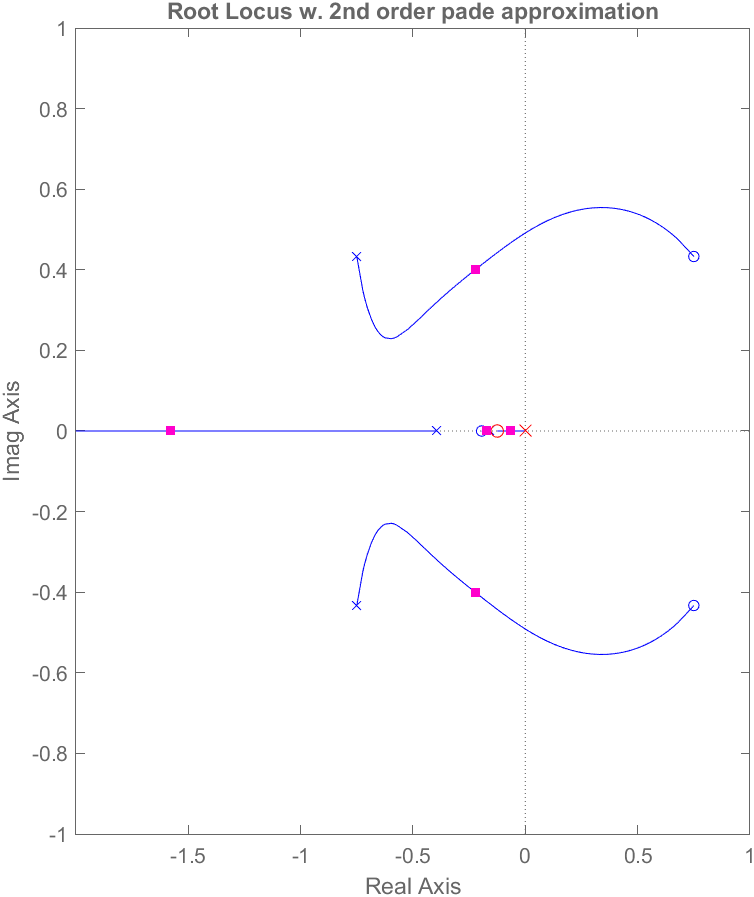
\includegraphics[height=4.8cm,width=\linewidth]{Topics/ControlStructure/Graphics/RootLocus_Pade2.png}
		\label{fig:RootLocus}
	\end{column}
\end{columns}
	Results in controller transfer function:
	\begin{equation}\label{eq:PIDTransferFunction}
	C(s) = \frac{K_ps+K_i}{s} = \frac{1.8s+0.225}{s}
\end{equation}
\end{frame}


\begin{frame}{Control Structure}{Step Response}
	\begin{figure}[h]
		\centering
		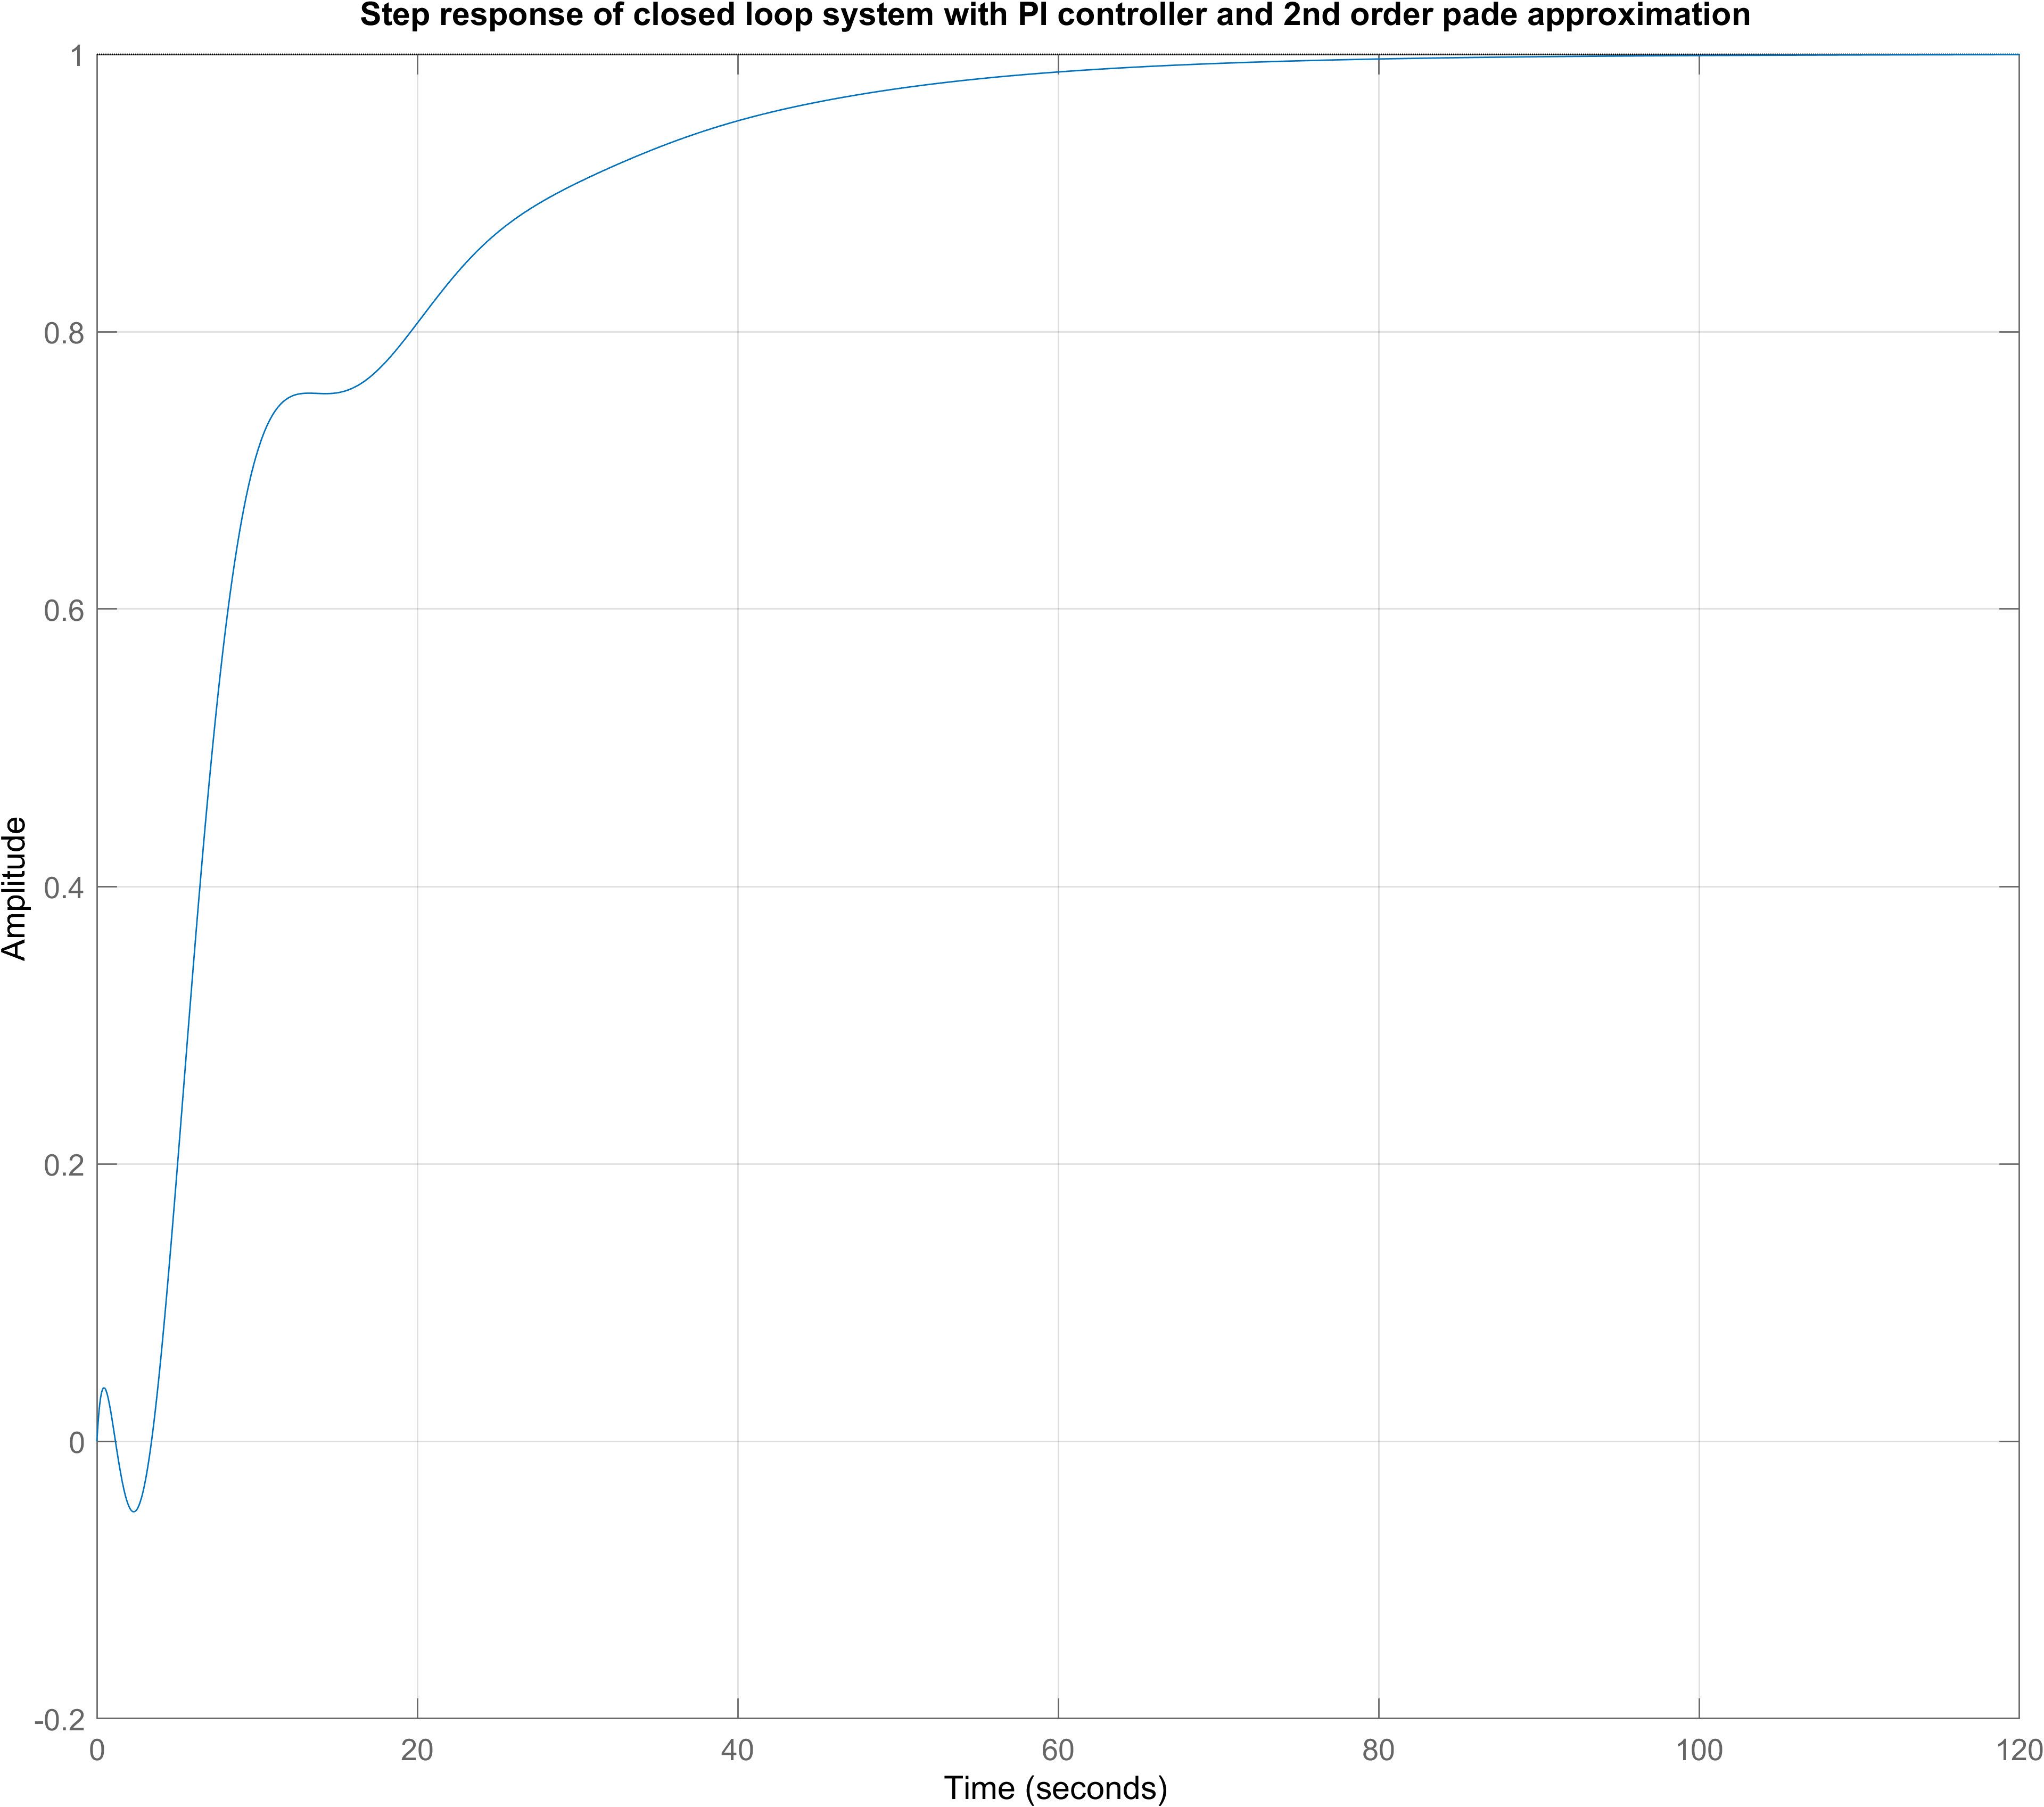
\includegraphics[height=6cm,width=0.6\linewidth]{Topics/ControlStructure/Graphics/StepResponse_Pade2.png}
		\label{fig:StepResponse_Pade2.png}
	\end{figure}

\end{frame}


\section{Optimal Control}

% motivation for creating this theme
\begin{frame}{Optimal Control}{General Optimal Control Problem}
	The basic structure of an optimal control problem is sketched in the language of calculus of variations.
	\begin{align}
		\dot{x} = &f(x,u,t) \label{eq:BasicOptimalFunction} \\ 
		x(t_0) = x_0, \ &x \in \mathbb{R}^n, \ u \in U \subseteq \mathbb{R}^m \label{eq:BasicOptimalDefinitions}
	\end{align}
	
	where $t \in \mathbb{R}$ is the time and $x,u$ are functions of $t$, with $U$ the set of admissible controls. \\
	\medskip
	Cost functional:
	\begin{equation}\label{eq:BolzaProblem}
		J = \mathcal{M}(x(T)) + \int_{0}^{T} \mathcal{L}(x(t),u(t)) dt
	\end{equation} 
\end{frame}
%%%%%%%%%%%%%%%%

%\begin{frame}{Linear-Quadratic Regulator}
% Let the dynamics of the (timevarying) system be given by:
%	\begin{equation}
%		\dot{x}(t) = A(t)x(t) + B(t)u(t) \label{eq:TimeVaryingLinearSystem}
%	\end{equation}
%
%	Cost functional:
%	\begin{equation}
%		J = \int_{t_0}^{t_1} \mathcal{L}(x(t),u(t)) dt + x^T(t_1)\mathcal{M}x(t_1)
%	\end{equation}
%	
%	Lagrangian:
%	\begin{equation}\label{eq:LQRLagrangian}
%		\mathcal{L}(x(t),u(t)) = x^T(t)Q(t)x(t) + u^T(t)R(t)u(t)
%	\end{equation}
%	
%	\begin{itemize}
%		\item Not time invariant!
%	\end{itemize}
%	
%\end{frame}

	%%%%%%%%%%%%%%%%
\begin{frame}{Infinite-Horizon Linear-Quadratic Regulator}
	The LQR time-invariant case with no terminal cost.\\
	System Dynamics:
	\begin{equation}
		\dot{x}(t) = Ax(t) + Bu(t) \label{eq:TimeInvariantLinearSystem}
	\end{equation}

	Cost functional:		
	\begin{equation}\label{eq:LagrangeProblem}
		J = \int_{t_0}^{\infty} \big(x^T(t)Qx(t) + u^T(t)Ru(t)\big)dt
	\end{equation} 

	State feedback control law:
	\begin{equation}\label{eq:InfLQRFeedbackLaw}
		u^*(t) = -R^{-1}B^TPx^*(t)
	\end{equation}
	
	$P$ is time-invariant and fullfills the \textit{algebraic Riccati equation}:
	
	\begin{equation}\label{eq:ARE}
		PA + A^TP + Q - PBR^{-1}B^TP = 0
	\end{equation}
\end{frame}

	%%%%%%%%%%%%%%%%
\begin{frame}{Tracking LQR and Integral Action}{Tracking LQR}
	 
	
	Let $\hat{x} = x-x_r$ and $\hat{u} = u-u_r$. Shifted coordinate system cost functional framed as an output tracking problem:
		
	
	\begin{equation}\label{eq:LagrangeProblemOutput}
		J = \int_{t_0}^{\infty} \big( \big(C^T\hat{x}^T\big) Q_y \big(C\hat{x}\big) + \hat{u}^TR\hat{u} \big) dt = \int_{t_0}^{\infty} \big(\hat{y}^TQ_y\hat{y} + \hat{u}^TR\hat{u}\big)dt
	\end{equation} 
	
	\begin{itemize}
		\item If linearised around some equilibrium point, these can be used as reference.
	\end{itemize}

\end{frame}


\begin{frame}{Tracking LQR and Integral Action}{Integral Action}
	States are extended with integral state $x_i$
	\begin{align}\label{eq:ClassicalIntegralAction}
		&u = -\bar{K}\bar{x} \\
		&\dot{\bar{x}} = \bar{A}\bar{x} + \bar{B}u + B_r r \\ 
		&y = \bar{C}\bar{x}\\
		&\bar{A} = \begin{bmatrix}A & 0 \\ -C & 0 \end{bmatrix}, \ \bar{B} = \begin{bmatrix} B \\ 0 \end{bmatrix}, \ B_r = \begin{bmatrix} 0 \\ 1 \end{bmatrix}, \ \bar{C} = \begin{bmatrix} C & 0 \end{bmatrix}\\
		& \bar{K} = -\begin{bmatrix} K & -K_i \end{bmatrix}
	\end{align}

	$K_i$ can be an awkward weight to choose.
\end{frame}

	%%%%%%%%%%%%%%%%
\begin{frame}{Velocity-Form LQR}
	Deviation variables:
	\begin{equation}\label{eq:VelocityVariables}
		\Delta x_k = x_k - x_{k-1}, \ \Delta y_k = y_k - r_k, \ \Delta u_k = u_k-u_{k-1}
	\end{equation}
	
	Extended vectors and matrices:
	\begin{equation} \label{eq1}
		\begin{split}
			& \tilde{\zeta}_k = \begin{bmatrix} \Delta x_k \\ \Delta y_k	\end{bmatrix}, \ \tilde{u}_k = \Delta u_k, \\
			&\tilde{A} = \begin{bmatrix} A & 0 \\ CA & I	\end{bmatrix}, \ 
			\tilde{B} = \begin{bmatrix} B \\ CB	\end{bmatrix}, \ \tilde{C} = \begin{bmatrix} 0 & I	\end{bmatrix}
		\end{split}
	\end{equation}

	Cost functional:
	\begin{equation}\label{eq:LagrangeProblemDeviation}
		J = \sum_{k_0}^{\infty} \big(\tilde{\zeta}^TQ\tilde{\zeta} + \tilde{u}^TR\tilde{u}\big)
	\end{equation}

	Origin regulation! If $\tilde{\zeta} \rightarrow 0 \Rightarrow  \Delta y \rightarrow 0 \Rightarrow  y \rightarrow r$.
\end{frame}

%Velocity-form dynamics:
%\begin{align}\label{eq:VelocityDynamics}
%	&\tilde{\zeta}_{k+1} = \tilde{A} \tilde{\zeta}_{k}  + \tilde{B}\tilde{u}_k \\
%	&\Delta y_k = \tilde{C}\tilde{x}_k
%\end{align}

\begin{frame}{Velocity-Form LQR}{Feedback Law}
	Control input applied at time k is:
	\begin{equation}\label{eq:ActualControlApplied}
		u^*(k) = \sum_{i=1}^{k} \Delta u^*(i)
	\end{equation}

	with
	\begin{equation}
		\tilde{K} = (\tilde{B}^TP\tilde{B}-R)^{-1}(\tilde{B}^TP\tilde{A})
	\end{equation}
\end{frame}


\begin{frame}{Velocity-Form LQR}{Disturbance-accommodating VF-LQR}

	Standard LQR does not accommodate exogenous inputs (such as the the model of the consumer demand flows) but can be modified to do so:
	\begin{equation}
		u(k) = \sum_{i=1}^{k} \Delta{u}^*(i) - B^\dagger \mathcal{B}\delta(i)
	\end{equation}
	
	where $B^\dagger$ is the Moore-Penrose pseudoinverse of $B$ and $\mathcal{B}$ is the disturbance input matrix.
\end{frame}


\section{Disturbance Estimator}
\begin{frame}
 \textbf{Objectives with the use of Kalman filte}
 \begin{itemize}
 	\item VF-LQR controller needs an estimate of the consumer demand.
 	\item The optimal estimator is the \textbf{Kalman Filter}.
 	\item Recursively finds optimal Kalman gain.
 	\item Kalman filter is also very interesting when from a leakage detection POV.  
 \end{itemize}
\end{frame}

	\begin{frame}{Water consumption data}
		\begin{itemize}
			\item Data of consumption pattern over a 35 day period obtained by CSK.  
		\end{itemize}
			 \begin{figure}[h!]
			\centering
			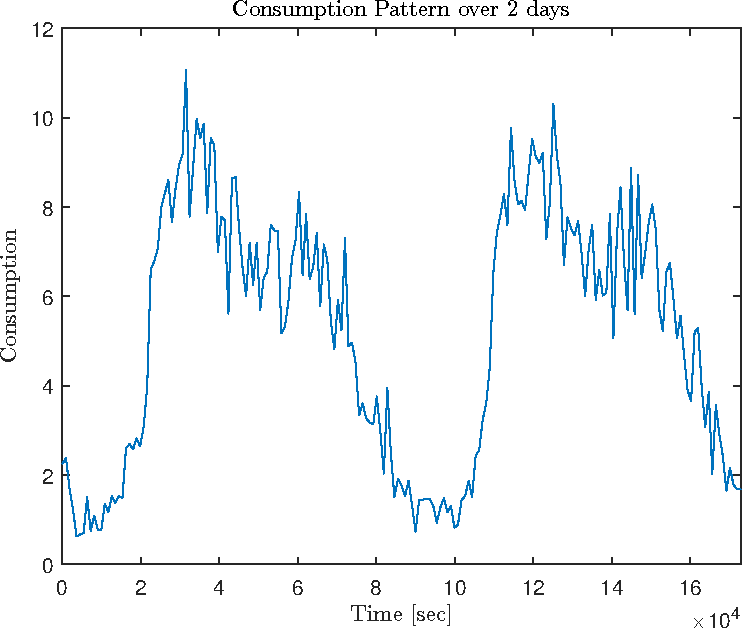
\includegraphics[width=0.6\textwidth]{Topics/KalmanEstimator/Graphics/ConsumptionPattern.pdf}
			\caption{Consumption pattern over two days}
			\label{fig:Consumption_Pattern}
		\end{figure}
	\end{frame}
	
	\begin{frame}{FFT of consumption pattern}
		\begin{itemize}
			\item Frequency analysis of the data. 
		\end{itemize}
	
		 \begin{figure}[h!]
			\centering
			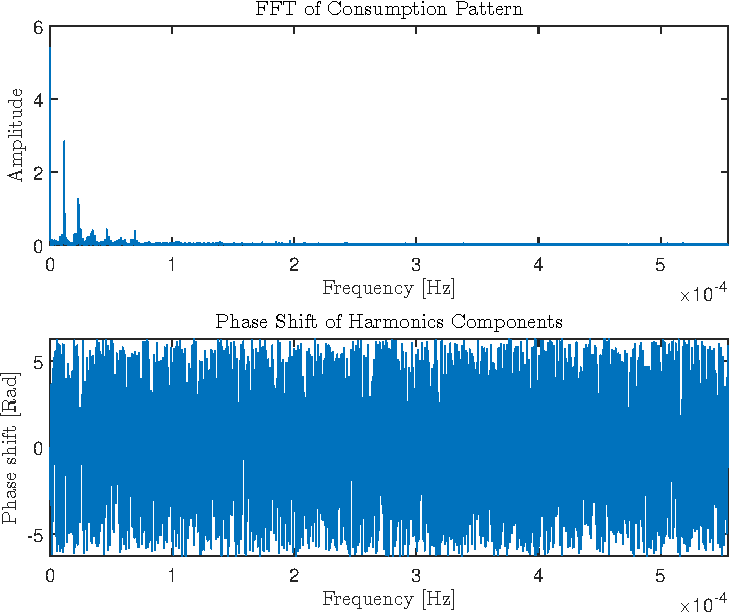
\includegraphics[width=0.6\textwidth]{Topics/KalmanEstimator/Graphics/FFT.pdf}
			\caption{Consumption pattern over two days}
			\label{fig:FFT_Consumption_Patter}
		\end{figure}
	
	\begin{itemize}
		\item Highest frequency contents at periods: DC, 24.05h, 12.03h, 8.02h and 5.99h. 
	\end{itemize}

	\end{frame}

%%%%%%%%%%%%%%%%%
	\begin{frame}{Approximation of consumption}
		
	\begin{itemize}
		\item Fourth order Fourier approximation of consumer demand:
	\end{itemize}
		
	\begin{equation} \label{eq:4th_order_approx}
		\begin{split}
			d_c(t) \approx& k_0 + k_1 cos(\omega_1 t + \phi_1) + k_2 cos(\omega_2 t + \phi_2)\\
			&+ k_3 cos(3\omega_3 t + \phi_3) + k_4 cos(4\omega_4 t + \phi_4)
		\end{split}
	\end{equation}

	\begin{itemize}
		\item We wish to model \ref{eq:4th_order_approx} as a state space model:
	\end{itemize}
		
			\begin{equation*}
			\begin{split}
				\dot{x}=Ax\\
				y=Cx
			\end{split}
		\end{equation*}	
	\end{frame}
%%%%%%%%%%%%%%%%%%%%%%%
\begin{frame}{State space representation}
	\begin{itemize}
		\item Need to represent the evolution of the "states" in the approximation as a linear combination of states.
		\item This can not be achieved using the current states.   
	\end{itemize}
	
\begin{equation} \label{eq:consump_A}
	\dot{x} = 
	\begin{bmatrix}
		0 & 0 & 0 & 0 & 0 \\
		0 & 0 & -\omega_1 & 0 & 0 \\
		0 & \omega_1 & 0 & 0 & 0 \\
		0 & 0 & 0 & 0 & -\omega_2 \\
		0 & 0 & 0 & \omega_2 & 0 
	\end{bmatrix}
	\begin{bmatrix}
		k_0 \\
		k_1 cos(\omega_1 t) \\
		k_1 sin(\omega_1 t) \\
		k_2 cos(\omega_2 t) \\
		k_2 sin(\omega_2 t) 
	\end{bmatrix}
\end{equation}

\begin{equation}
	y = \begin{bmatrix} 1 & 1 & 0 & 1 & 0 \end{bmatrix} 
	\begin{bmatrix}
		k_0 \\
		k_1 cos(\omega_1 t) \\
		k_1 sin(\omega_1 t) \\
		k_2 cos(\omega_2 t) \\
		k_2 sin(\omega_2 t) 
	\end{bmatrix}
\end{equation}

	\begin{itemize}
	\item Fourth order doesn't fit the page..
\end{itemize}
\end{frame}

%%%%%%%%%%
	\begin{frame}{Model vs. data}
\begin{itemize}
		\item The model compared to the real data - shown over 2 days. 
\end{itemize}
		\begin{figure}[h!]
			\centering
			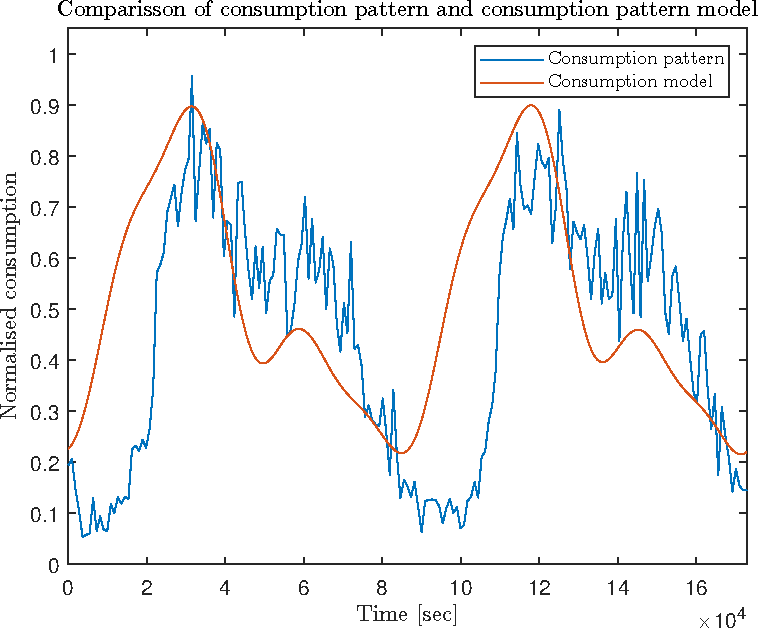
\includegraphics[width=0.6\textwidth]{Topics/KalmanEstimator/Graphics/Comparisson.pdf}
			\caption{Comparison of raw historical data, and model}
			\label{fig:Comparison}
		\end{figure}
	\begin{itemize}
		\item The model follows the visual trend in real data.
	\end{itemize}	
	\end{frame}

\begin{frame}{The Kalman Filter}
	\textbf{Considerations when designing the KF.}
	\begin{itemize}
		\item Stiffness of the filter
	\end{itemize}
\end{frame}
%
\section{Network effects}
\begin{frame}{Network Effects}
	\begin{itemize}
		\item Outer loop
		\begin{itemize}
			\item Central control unit
			\item Transmit data
		\end{itemize}
		\item Urban environment
		\begin{itemize}
			\item Packet loss scaling with distance
			\item $ 60\% $ or more expected at 20 km
		\end{itemize}
		\item Try-Once-Discard protocol used
		\begin{itemize}
			\item Packet loss -> 0 control input
		\end{itemize}
	\end{itemize}
	\begin{figure}[h!]
	\centering
	\resizebox{0.9\columnwidth}{!}{
			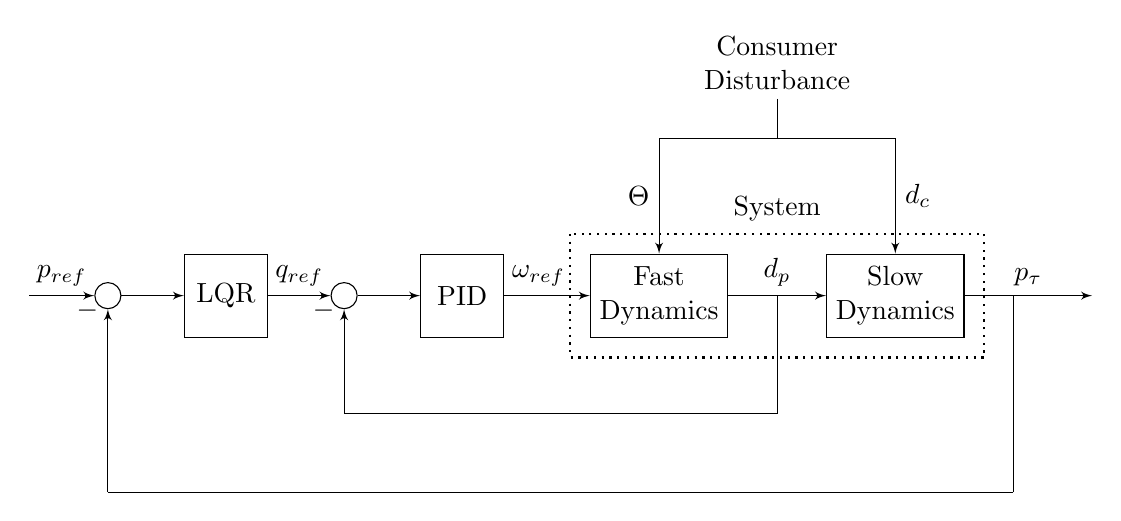
\begin{tikzpicture}[auto, node distance=2.5cm,>=latex']
	% ========================== Nodes ============================
	% Nodes in upper vertical line
	\node [input, name=rinput] (rinput) {};
	\node [sum, right of=rinput] (sum1) {};
	\node [block, right of=sum1, node distance = 1.5cm] (LQR) {LQR};
	\node [sum, right of=LQR, node distance =
	1.5cm] (sum2) {};
	\node [block, right of=sum2, node distance = 1.5cm] (PID){PID};
	\node [block, right of=PID, align=center] (Fast){Fast\\Dynamics};
	\node [block, right of=Fast, node distance = 3cm, align=center] (Slow){Slow\\Dynamics};
	\node [output, right of=Slow] (output) {};
	
	% Nodes for inner feedback
	\node [tmp, right of=Fast, node distance = 1.5cm] (tmp0){};
	\node [tmp, below of=tmp0, node distance = 1.5cm] (tmp1){};
	\node [tmp, below of=sum2, node distance = 1.5cm] (tmp2){};
	
	% Nodes for outer feedback
	\node [tmp, right of=Slow, node distance = 1.5cm] (tmp10){};
	\node [tmp, below of=tmp10,node distance = 2.5cm] (tmp11){};
	\node [tmp, below of=sum1, node distance = 2.5cm] (tmp12){};
	
	% Nodes for Disturbance
	\node [tmp, above of=tmp0, node distance = 2.5cm] (tmp20){};
	\node [tmp, above of=tmp0, node distance = 2cm] (tmp21){};
	\node [tmp, above of=Fast, node distance = 2cm] (tmp22){};
	\node [tmp, above of=Slow, node distance = 2cm] (tmp23){};
	
	\draw[thick, dotted] ($(Fast.north west)+(-0.25, 0.25)$) rectangle  ($(Slow.south east)+(0.25, -0.25)$);
	\node[above of =tmp0, node distance =1.1cm](sys_txt) {System};
	
	% ========================== Lines ============================
	
	% Lines in upper vertical part of block diagram
	\draw [->] (rinput) -- node{$p_{ref}$} (sum1);
	\draw [->] (sum1) --node[name=z,anchor=north]{} (LQR);
	\draw [->] (LQR) -- node{$ q_{ref} $}(sum2);
	\draw [->] (sum2) -- (PID);
	\draw [->] (PID) -- node[pos=0.4]{$ \omega_{ref} $}(Fast);
	\draw [->] (Fast) -- node{$d_p$}(Slow);
	\draw [->] (Slow) -- node{$p_{\tau}$}(output);	
	
	% Lines for inner feedback
	\draw [-] (tmp0) -- (tmp1);
	\draw [-] (tmp1) -- (tmp2);
	\draw [->] (tmp2) -- node[pos=0.99]{$ - $}(sum2);
	
	
	% Lines for outer feedback
	\draw [-] (tmp10) -- (tmp11);
	\draw [-] (tmp11) -- (tmp12);
	\draw [->] (tmp12) -- node[pos=0.99]{$ - $}(sum1);
	
	
	% Lines for disturbance
	\draw [-] (tmp20)node[above, align=center]{Consumer \\ Disturbance} -- (tmp21);
	\draw [-] (tmp21) -- (tmp22);
	\draw [-] (tmp21) -- (tmp23);
	\draw [->] (tmp22) -- node[left, pos = 0.5]{$\Theta$}(Fast);
	\draw [->] (tmp23) -- node[pos = 0.5]{$ d_c $}(Slow);
	
	
\end{tikzpicture}
}
	\label{fig:tikzControlStructure}
\end{figure}
\end{frame}

\begin{frame}{For Specific Packet Loss}
	\begin{itemize}
		\item Assuming $ 60\% $ as upper bound for loss, $ \alpha $, the condition for mean squre stability is:
	\begin{equation}\label{eq:HuStabCondition}
		\mathcal{S}\Big(\alpha A \otimes A + (1-\alpha)(A-BK) \otimes (A-BK) \Big) < 1
	\end{equation}
		\item The propagation matrix of the states covariance
	\begin{equation}\label{eq:HuStabCondition}
		\alpha A \otimes A + (1-\alpha)(A-BK) \otimes (A-BK) 
	\end{equation}
		\item For stability this must hold 
	\begin{equation}
		\lim_{k \rightarrow \infty} \text{E}[x(k)^2] = 0
	\end{equation}
		\item We get $\mathcal{S} = 0.9453 $
	\end{itemize}
\end{frame}	
	
\begin{frame}{For Any Packet Loss}
	\begin{itemize}
		\item Largest possible bound for packet drop, $ \alpha $, where the system will be marginal stable
		\begin{equation}\label{eq:VMatrix}
			\begin{gathered}
				\Xi = \frac{1}{\lVert\sigma_+(V)\rVert_\infty} \\
				V = \begin{bmatrix} (S\otimes\hat{S}+\hat{S} \otimes S)(I - S\otimes S)^{-1} & \hat{S}\otimes\hat{S} \\ (I - S\otimes S)^{-1} & 0 \end{bmatrix} \\
				S = \left(A-BK\right) \otimes \left(A-BK\right), \quad \hat{S} = A \otimes A - S
			\end{gathered}
		\end{equation}
		\item Plugging in the LQR matrices and no control
		\begin{equation}
			\begin{split}
				\lim_{\tilde{K}\rightarrow 0} \Big(\alpha \tilde{A} \otimes \tilde{A} + (1-\alpha)(\tilde{A}-\tilde{B}\tilde{K}) \otimes (\tilde{A}-\tilde{B}\tilde{K}) \Big) \\
				= \Big(\alpha \tilde{A} \otimes \tilde{A} + (1-\alpha)\tilde{A} \otimes \tilde{A}\Big)	
			\end{split}
		\end{equation}
	\end{itemize}
\end{frame}	

\begin{frame}{For Any Packet loss}
	\begin{itemize}
		\item asddas
		\begin{equation}
			\begin{split}
				\forall \alpha \in \{0 \dots 1\}: \quad \Big(\alpha \tilde{A} \otimes \tilde{A} + (1-\alpha)\tilde{A} \otimes \tilde{A}\Big) \\
				= \tilde{A}\otimes\tilde{A} 
				= \begin{bmatrix}  
					1 & 0 & 0 & 0 \\
					1 & 1 & 0 & 0 \\
					1 & 0 & 1 & 0 \\
					1 & 1 & 1 & 1	
				\end{bmatrix}
			\end{split}
		\end{equation}
		\item Thus the EWR is marginally stable for any packet loss -> $ \mathcal{S}={1, 1, 1, 1}  $
	\end{itemize}
\end{frame}


%
%\section{Results}
%\input{Topics/XX/XX}















% ======================================================================




\section{References}
\begin{frame}{References}
	\bibliographystyle{ieeetran}
	\bibliography{../RefLib/CA7Projekt.bib}
\end{frame}

{\aauwavesbg
\begin{frame}[plain,noframenumbering]
  \finalpage{Open for questions!}
\end{frame}}
%%%%%%%%%%%%%%%%

\end{document}
